\part{From Tensors to Networks}
\label{sec:tensor}

Tensors are a mathematical concept that encapsulates and generalizes the idea of
multilinear maps, i.e.~functions of multiple parameters that are linear with respect to every parameter.
A tensor network is simply a countable collection of tensors connected by contractions.
{\bf Tensor network methods} is the term sometimes given to the entire collection of associated tools, which are regularly employed in modern quantum information science, condensed matter physics, mathematics and computer science.  
 
Tensor networks come with an intuitive graphical language that can be used in formal reasoning and in proofs. 
This diagrammatic language found applications in physics at least as early as the 1970s by Roger Penrose~\cite{Penrose}.
Tensor network theory has recently seen many advancements and adaptations to different domains of physics, mathematics and computer science.
An important milestone was David Deutsch's use of the diagrammatic notation in quantum computing,
developing the \emph{quantum circuit} (a.k.a.~quantum computational networks as Deutsch would call them)
model~\cite{Deutsch73}.
Quantum circuits are a special class of tensor networks, in which the arrangement of the tensors and their types are restricted.
%However, these topics fit together nicely, recovering one from the other by lifting or dropping specific restrictions.
A related diagrammatic language slightly before that is due to Richard Feynman~\cite{Fey86}.
The quantum circuit model---now well over two decades old---is widely used
to describe quantum algorithms and their experimental implementations,
to quantify the resources they use (by e.g.~counting the quantum gates required),
to classify the entangling properties and computational power of specific gate families, and more.

There is growing excitement concerning numerical algorithms that 
perform tensor contractions.  These algorithms are important in condensed matter physics and beyond.  There are many reviews and surveys devoted to this important direction---see~\cite{2014AnPhy.349..117O, Vidal2010, MPSreview08, TNSreview09, 2011AnPhy.326...96S, 2010arXiv1006.0675S, Schollw, 2014EPJB...87..280O,2013arXiv1308.3318E,2011JSP...145..891E, 2016arXiv160303039B, MAL-059, Pervishko_2019, MAL-067,2017arXiv170809213R}, as well as, {\it Tensor Networks in a Nutshell}, which I wrote with Ville Bergholm \cite{biamonte2017tensor}. 
Some of the best known applications of tensor networks are 1D Matrix Product States (MPS),  Tensor Trains (TT)~\cite{Oseledets2011}, Tree Tensor Networks (TTN),
the Multi-scale Entanglement Renormalization Ansatz (MERA), Projected Entangled Pair States (PEPS)---which generalize matrix product states to higher dimensions---and various other renormalization methods~\cite{Vidal2010, MPSreview08, TNSreview09, 2011AnPhy.326...96S, 2009PhRvL.102e7202H, 2013arXiv1308.3318E, MAL-059}.  
The excitement is based on the fact that certain
classes of quantum systems can now be simulated more efficiently, studied in greater detail,
and this has opened new avenues for a greater understanding of certain physical systems.  The concept is to factor a quantum state ~$\psi$ into various network structures, as follows.  

\begin{center}
    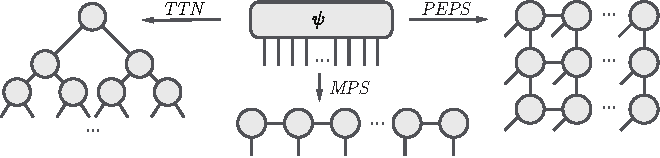
\includegraphics{tensor-types-2} 
\end{center}

These methods approximate a complicated quantum state using a tensor network with a simplistic, regular structure---essentially applying lossy data compression that preserves the most salient properties of the quantum state.  The method is known to efficiently work for certain classes of ground and thermal states. 

We assume that most readers will have a basic understanding of some quantum theory, linear algebra and tensors.




\section{Penrose Graphical Notation for Tensor Networks} 

We will present a variant of the graphical notation used by Penrose \cite{Penrose, Penrose67, road}.  This book presents the modern incarnation of these ideas, building on four ingredients: (i) modern tensor networks as they appear in condensed matter physics; (ii) quantum circuits and their graphical language \cite{NC}; (iii) aspects of categorical quantum mechanics  \cite{Coecke2017} as they describe quantum circuits \cite{CD, redgreen} as well as (iv) the graphical language of digital circuits.  

The output of this merger is an increasingly popular collection of ideas related to the application of tensor networks to quantum information and quantum computation following largely \cite{CTNS, BB11}.  The notation matches quantum circuit notation and the presentation should hopefully be approachable for a wide audience of modern quantum information scientists.  Indeed, the techniques do differ from any of the respective ingredients we have mixed together; so any of the above listed communities---(i), (ii), (iii), (iv)---should go away after reading these notes with new techniques.  

\begin{paragraph}{Tensor Network}
Tensors
\begin{marginfigure}
\centering
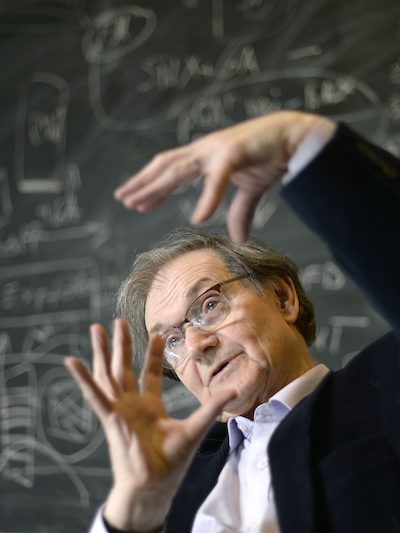
\includegraphics[width=5\xxxscale]{PenroseQ}
\caption{``\textit{It now ceases to be important to maintain a distinction 
between upper and lower indices.}''
{-- Roger Penrose, 1971 \cite{Penrose}.}}
\end{marginfigure}
can be thought of as indexed multi-dimensional arrays of complex numbers with respect to a fixed standard basis. 



\begin{definition}
 Let $\2 X, \2 Y, \2 Z$ be finite-dimensional complex Hilbert spaces,  ${\mathcal L}(\2X,\2Y)$ is the space of bounded linear operators $A: \2 X\rightarrow \2 Y$ with ${\mathcal L}(\2X)\equiv {\mathcal L}(\2X,\2X)$.
\end{definition}
For example, consider the Hilbert space $\2 X\cong \C^d$, where as is typical in modern quantum theory, we choose our standard basis to be the \emph{computational basis}
$$ 
\{\ket{i}\,:\, i=0,...,d-1\}.
$$ 
Then in Dirac notation a vector $\ket{v}\in \2 X$ is a 1st-order tensor which can be expressed in terms of its tensor components $v_i:=\braket{i}{v}$ with respect to the standard basis as $\ket{v}=\sum_{i=0}^{d-1} v_i\ket{i}$. Similarly one can represent linear operators on this Hilbert space, $A\in {\mathcal L}(\2 X)$,  as 2nd-order tensors with components $A_{ij}:= \bra{i}A\ket{j}$ as $A = \sum_{i,j=0}^{d-1} A_{ij} \ketbra{i}{j}$.

Hence, in Dirac notation the number of indices of a tensors components more define what we called a tensors \emph{order}. Vectors $\ket{v}\in \2 X$ refer to tensors which only have \emph{ket} ``$\ket{i}$'' basis elements, vectors in the dual vector space $\bra{u}\in \2 X^\dagger$ (or more typically denoted $\2X^\star$ or $\2X^*$) refer to those with only \emph{bras} ``$\bra{i}$'', and linear operators on $A\in \2 {\mathcal L}(\2 X)$ refer to tensors with a mixture of kets and bras in their component decomposition.

\begin{remark}
Like Penrose, we use the word \emph{valence} or \emph{order} instead of \emph{rank} when referring to the number of indices on a tensor, since rank is used elsewhere.  A tensor with $n$ indices up and $m$ down is called a valence-$(n,m)$ tensor and sometimes a valence-$k$ tensor for $k=n+m$. 
\end{remark}

\begin{remark}
The concurrent evaluation of all indices returns a complex number.  This is called total or full contraction.
\end{remark}

\begin{remark}
The idea of representing quantum states, operators and maps (etc.) diagrammatically is credited to works by Penrose and is sometimes referred to as \textit{Penrose graphical notation} or \textit{string diagrams}.  Though Penrose unquestionably pioneered many of the applications and uses of the language and deserves credit, Arthur Cayley developed much earlier variants of graphical languages. 
\end{remark}



We mostly adhere to Penrose's notation of representing states (vectors) and effects (dual-vectors) as triangles, linear operators as boxes, and scalars as diamonds, as found in Illustration~\ref{fig:ketbramat}. Here each index corresponds to an open wire on the diagram and so we may define higher order tensors with increasingly more wires. The number of wires is then the order of the tensor, with each wire acting on a separate vector space $\2 X_j$.
% FIGURE - BASIC TENSORS

\begin{myfullpage}
\begin{illexample}[Graphical depiction of elementary tensors]
\label{sfig}
 Non-zero scalars (d) are also represented as `blank' on the page.  We represent vectors (states) and dual-vectors (effects) as triangles, linear operators as boxes, and scalars as diamonds, with each index of the tensor depicted as an open wire on the diagram. The orientation of the wires determines the type of tensor, in our convention the open end of the wires point to the left for vectors, right for dual-vectors, and both left and right for linear operators.
 \begin{center} 
\begin{tabular}{cccc}
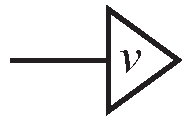
\includegraphics[width=0.11\textwidth]{fig2a} &
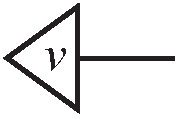
\includegraphics[width=0.11\textwidth]{fig2b} &
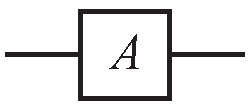
\includegraphics[width=0.145\textwidth]{fig2c} &
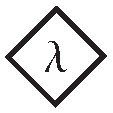
\includegraphics[width=0.085\textwidth]{fig2d}  
\\
\footnotesize{(a) Vector $\ket{v}\in\2 X$} &
\footnotesize{(b) Dual-vector $\bra{v}\in \2 X^\dagger$}&
\footnotesize{(c) Linear Operator $A\in \2 {\mathcal L}(\2 X)$}&
\footnotesize{(d) Scalar $\lambda\in\C$} 
\\~\\
& 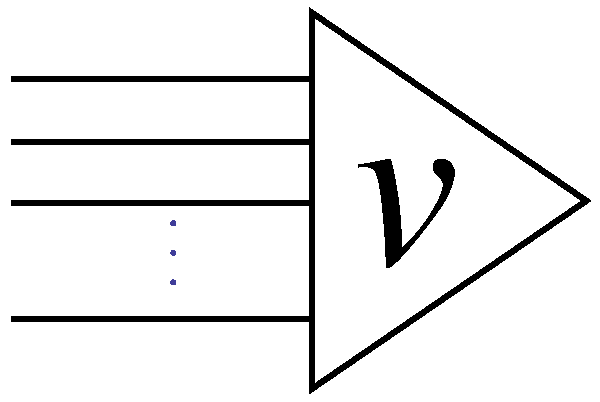
\includegraphics[width=0.1\textwidth]{fig2e} &
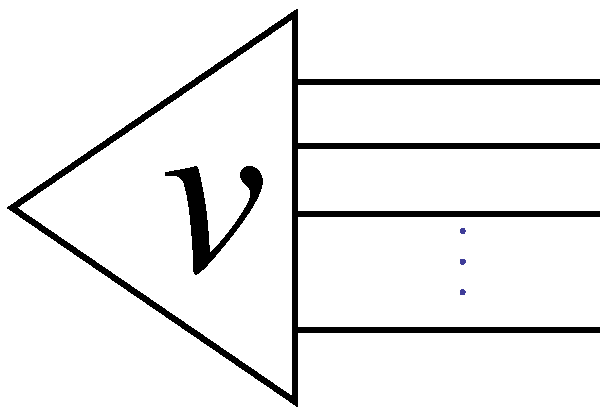
\includegraphics[width=0.1\textwidth]{fig2f}  &
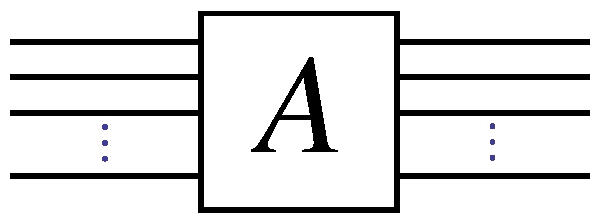
\includegraphics[width=0.145\textwidth]{fig2g}
\\
& \footnotesize{(e) Vector $\ket{v}\in \bigotimes_{i=1}^n \2 X_i$} &
\footnotesize{(f) Dual-vector $\bra{v}\in \bigotimes_{i=1}^n \2 X^\dagger_i$} &
\footnotesize{(g) Linear operator $A$:}
\\
& & &
\footnotesize{$\2 \bigotimes_{i=1}^n \2 X_i \rightarrow \bigotimes_{j=1}^m \2 X_j$}
\end{tabular}
\end{center} 

%%%%%%%%%%%%%%%%%%%%%%
\begin{comment}
\begin{figure*}[H] \centering
      \vspace{-1em}
 	\subfloat[Vector $\ket{v}\in\2 X$]{
		\label{sfig:ket}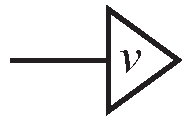
\includegraphics[width=0.11\textwidth]{fig2a}}
		\hspace{0.5em}
  	\subfloat[Dual-vector $\bra{v}\in \2 X^\dagger$]{
		\label{sfig:bra}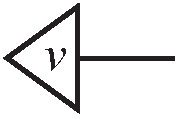
\includegraphics[width=0.11\textwidth]{fig2b}}
		\hspace{0.5em}
   	\subfloat[Linear Operator $A\in \2 {\mathcal L}(\2 X)$]{
		\label{sfig:mat}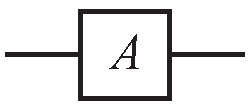
\includegraphics[width=0.145\textwidth]{fig2c}}
		\hspace{0.5em}
   	\subfloat[Scalar $\lambda\in\C$]{
		\label{sfig:scalar}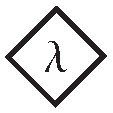
\includegraphics[width=0.085\textwidth]{fig2d}}
		\hspace{1em}
	\subfloat[Vector $\ket{v}\in \bigotimes_{i=1}^n \2 X_i$]{
		\label{sfig:gket}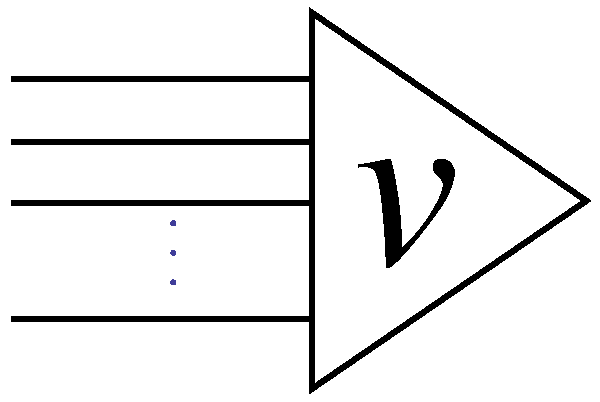
\includegraphics[width=0.1\textwidth]{fig2e}}
		\hspace{1em}
  	\subfloat[Dual-vector $\bra{v}\in \bigotimes_{i=1}^n \2 X^\dagger_i$]{
		\label{sfig:gbra}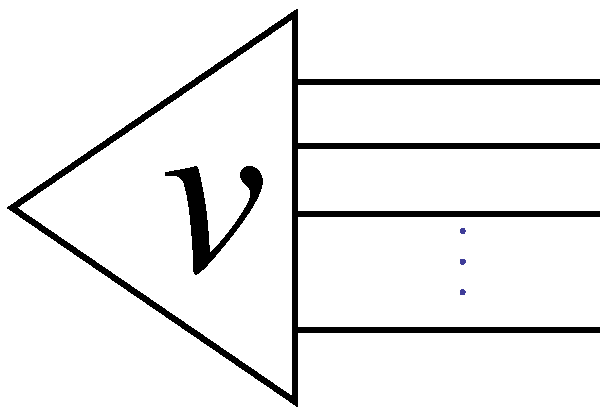
\includegraphics[width=0.1\textwidth]{fig2f}}
		\hspace{1em}
   	\subfloat[Linear operator $A:\2 \bigotimes_{i=1}^n \2 X_i \rightarrow \bigotimes_{j=1}^m \2 X_j$]{
		\label{sfig:gmat}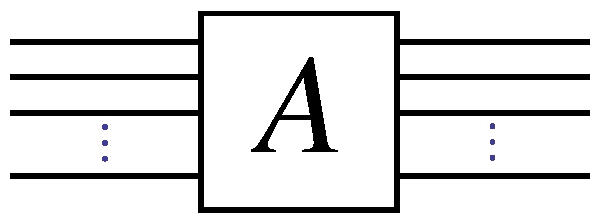
\includegraphics[width=0.145\textwidth]{fig2g}}
% \caption{
 \end{figure*}
 \end{comment}
 %%%%%%%%%%%%%%%%%%%%%%%%%%
  \label{fig:ketbramat}
\end{illexample}
\end{myfullpage}
\end{paragraph}

It is typical in quantum physics to think of a tensor as an indexed multi-array of numbers.\mn{Abstract index notation is a mathematical notation for tensors that uses indices as place holders identifying space(s), rather than their components in a particular basis.}  For instance,  
\begin{center}
 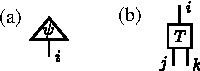
\includegraphics[width=6\xxxscale]{tensors-example}
\end{center}
represent the tensor (a) $\psi_i$ in the space $\2 H_i$ and (b) $T^i_{~jk}$ in the space 
$$
\2H^i\otimes \2H_j \otimes \2 H_k
$$
% or written $\2H^\star\otimes \2H \otimes \2 H$ 
respectively.  

\begin{remark}[Diagram convention---top to bottom, or right to left] 
Open wires pointing towards the top of the page, correspond to upper indices (bras), open wires pointing towards the bottom of a page correspond to a lower indices (kets).  For ease of presentation, we will often rotate this convention $90$ degrees counterclockwise.


\textcolor{red}{Fix the convention, it might just need to fix illustration 1.1}
\end{remark}
% get degree symbol to work in latex.  

%The alternative approach would be to attach the basis element to the tensor (e.g. $\psi^i e_i$ and use the double sum convention), but when working with such objects, this information is almost always redundant and/or cumbersome.
There are three specific tensors that (essentially) play the role of Kronecker's delta.  These tensors allow for (i) tensor index contraction by diagrammatic connection, (ii) raising and lowering indices, and (iii) they give rise to a duality between maps, states and linear maps in general.  The bijection induced by bending wires, is sometimes called \textit{Penrose Duality}, after its inventor \cite{Penrose}.  As in \cite{Penrose}, these three tensors are given diagrammatically as 
\begin{center}
 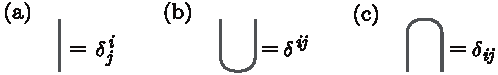
\includegraphics[width=12\xxxscale]{delta}
\end{center}

By thinking of these tensors in terms of their components, e.g.\ $\delta_{ij}=1-(i-j)^2$ for $i,j=0,1$, we note that 
\begin{equation}\label{eqn:delta}
 \I = \sum_{ij}\delta^i_j\ket{i}\bra{j}=\sum_k\ket{k}\bra{k}, 
\end{equation}

\begin{equation}\label{eqn:delta-bell}
 \ket{00}+\ket{11}+\dots +\ket{nn} = \sum_{ij} \delta^{ij}\ket{ij}=\sum_k\ket{kk},
\end{equation}

\begin{equation}\label{eqn:delta-effect}
 \bra{00}+\bra{11}+\dots + \bra{nn} = \sum_{ij} \delta_{ij}\bra{ij}=\sum_k\bra{kk}. 
\end{equation}
Here the identity map in (a) corresponds to \eqref{eqn:delta}, the cup (b) to \eqref{eqn:delta-bell} and the cap (c) to \eqref{eqn:delta-effect}.  The relation between these three equations is given by bending wires.  In a real-valued basis, bending a wire corresponds to changing a bra to a ket, and vise versa.  

The contraction of two tensor indices diagrammatically amounts to joining two wires.  Given tensors 
$T^i_{~jk}$, $A^l_{~n}$ and $B^q_{~m}$ we form a contraction between indices by assigning them the same variable:
\be 
\sum_{j,k}T^i_{~jk}A^j_{~n}B^k_{~m} \bydef \Gamma^i_{~nm},
\ee 
where the tensor $\Gamma^i_{~nm}$ is introduced per definition to simplify notation.  As a linear map, in quantum physics notation, this is typically expressed in equational form as 
\be 
\Gamma = \sum_{inm}\Gamma^i_{~nm}\ket{i}\bra{nm} = \sum_{ijknm} T^i_{~jk}A^j_{~n}B^k_{~m}\ket{i}\bra{nm}. 
\ee 
So connecting tensors by a wire is given by a sum over a shared internal variable. This is reminiscent of multiplying by $\delta$ function: for example multiplying $T^i_{~jk}A^l_{~n}B^q_{~m}$ by $\delta^j_l\delta^k_q$ yeilds, 
\begin{equation}
    \sum_{j,l,k,q}T^i_{~jk}A^l_{~n}B^q_{~m}\delta^j_l\delta^k_q = \sum_{l,q} T^i_{~lq}A^l_{~n}B^q_{~m}.  
\end{equation}

\begin{remark}
Cups and caps appear on page 231 of {\it Applications of Negative Dimensional Tensors} by Roger Penrose \cite{Penrose}. The composition of cups and caps is the identity; known as the snake equation and also found on page 231 of \cite{Penrose}. 
\end{remark}



\subsubsection*{Connection to quantum computing notation}
As mentioned, tensors are multilinear maps.
They can be expanded in any given basis, and expressed in
terms of their components.
In quantum information science one often introduces a \emph{computational basis}
$\{\ket{k}\}_k$
for each Hilbert space
and expands the tensors in it, using kets ($\ket{~}$) for vectors and bras ($\bra{~}$) for dual vectors:
\be 
T = \sum_{ijk}T\indices{^i_{jk}}\ket{i}\bra{jk}.
\ee 
Here $T\indices{^i_{jk}}$ is understood
not as abstract index notation but as the actual components of the
tensor in the computational basis.
In practice there is little room for confusion.
The Einstein summation convention is rarely used in quantum information science,
hence we write the sum sign explicitly.


So far we have explained how tensors are represented in tensor diagrams,
and what happens when wires are connected. The ideas are concluded by four examples; we urge the reader to work through the examples and check the results for themselves.

The first example introduces a familiar structure from linear algebra in tensor form.
The next two examples come from quantum entanglement theory---see connecting
tensor networks with invariants~\cite{BBL11, 2014SIGMA..10..095C}.
The fourth one showcases quantum circuits, a subclass of tensor networks
widely used in the field of quantum information.
The examples are chosen to illustrate properties of tensor networks and should be self-contained.

\begin{remark}
We occasionally will work with equality up to a scalar when manipulating tensor diagrams by hand. This is common and typically amounts to loss of (unit) normalization.  In quantum theory, a global phase is undetectable.  Hence it is common to consider an equivalency class where $\ket{\psi}$ and $e^{\imath \phi}\ket{\psi}$ are equivalent. This is called working in the {\it unit gauge}: in tensor networks we sometimes work in the {\it scalar gauge}, $\mathbb{C}/\{0\}$. This amounts to mapping numbers picked up during calculation as 
$$
\mathbb{C}/\{0\}\rightarrow 1
$$ 
and representing the unit $1$ as a blank on the page. 
\end{remark}

\begin{example}[The $\epsilon$ tensor]\label{ex:epsilon}
A tensor is said to be fully antisymmetric if swapping any pair of
indices will change its sign: $A_{ij} = -A_{ji}$.
The $\epsilon$ tensor is used to represent the fully antisymmetric Levi-Civita
symbol, which in two dimensions can be expressed as
\begin{equation}
 \epsilon_{00}=\epsilon_{11}=0, \qquad
 \epsilon_{01}=-\epsilon_{10}=1.
\end{equation}

The $\epsilon$ tensor can be used to compute the determinant of a matrix. In two dimensions we have
\be
\det(S) = \epsilon_{ij} S\indices{^i_0} S\indices{^j_1}.
\ee
Using this we obtain
\begin{center}
 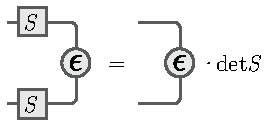
\includegraphics{epsilon}
\end{center}
as can be seen by labeling the wires in the diagram.
In equational form this is
\begin{equation}
\epsilon_{ij} S\indices{^i_m} S\indices{^j_n} = \det(S) \: \epsilon_{mn}.
\end{equation}

In terms of quantum mechanics, $\epsilon$ corresponds to the two-qubit
singlet state:
\be\label{eqn:singlet}
\frac{1}{\sqrt{2}} \ket{\epsilon} = \frac{1}{\sqrt{2}}(\ket{01}-\ket{10}).
\ee
This quantum state is invariant under any transformation of the form $U \otimes U$, where $U$~is a $2\times 2$ unitary,
as it only gains an unphysical global phase factor~$\det(U)$.

\end{example}


\begin{example}[Concurrence and entanglement]\label{ex:concurrence}
Given a two-qubit pure quantum state $\ket{\psi}$,
its \emph{concurrence}
$C(\psi) = |C'(\psi)|$
is the absolute value of the following tensor network expression~\cite{concurrence}:
\begin{center} \label{fig:con}
% Should have different name - PS
% \includegraphics[width=0.36\textwidth]{con} - PS
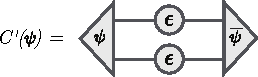
\includegraphics[width=0.36\textwidth]{con-ps}
\end{center}
Here $\overline{\psi}$ is the complex conjugate of~$\psi$ in the computational basis.
The concurrence is an entanglement monotone, a function from states to
nonnegative real numbers that measures how entangled the state is.
$\ket{\psi}$ is entangled if and only if
the concurrence is greater than zero.

Consider now what happens when we act on $\ket{\psi}$ by an arbitrary local unitary operation, i.e.
$$
\ket{\psi'} = (U_1 \otimes U_2) \ket{\psi}.
$$
Using the result of Example~\ref{ex:epsilon} we obtain
\begin{equation}
    C\left((U_1\otimes U_2) \ket{\psi}\right) = C(\psi) |\det(U_1) \det(U_2)|.
\end{equation}
Due to the unitarity 
$$
|\det U_1| = |\det U_2| = 1,
$$
which means that the value of the concurrence
is \emph{invariant} (i.e.~does not change) under local unitary transformations.
This is to be expected, as local unitaries cannot change the amount of entanglement in a quantum state.

%We will revisit concurrence in Example~\ref{ex:con-2}.

More complicated invariants can also be expressed as tensor networks~\cite{BBL11}.
We will leave it to the reader to write the following network as an algebraic expression:
\begin{center}
 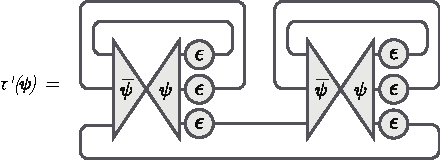
\includegraphics[width=0.6\textwidth]{3-tangle-II}
\end{center}
If $\ket{\psi}$ is a 3-qubit quantum state,
$\tau(\psi) = 2 |\tau'(\psi)|$ represents the entanglement invariant known as the 3-tangle~\cite{2000PhRvA..61e2306C}.
It is possible to form invariants also without using the epsilon tensor.  For example,
the following expression represents the 3-qubit entanglement invariant known as the Kempe invariant~\cite{kempe}:
\begin{equation}\label{eqn:kempe}
K(\psi) = \psi^{ijk}~\overline{\psi}_{ilm}~\psi^{nlo}~\overline{\psi}_{pjo}~\psi^{pqm}~\overline{\psi}_{nqk}.
\end{equation}
The studious reader would draw the equivalent tensor network.
\end{example}


\begin{example}[Quantum circuits] \label{ex:circuits-1}\marginnote{{\it ``I learned very early the difference between knowing the name of something and knowing something.''} --- Richard P.~Feynman, co-discover (with Norman Margolus) of the \CNOT- a.k.a.~Feynman-gate.}

Quantum circuits are a restricted subclass of tensor networks that is widely used in the field of quantum information and is the subject of \S~\ref{sec:btn}. In a quantum circuit diagram each horizontal wire represents the Hilbert space associated with a quantum subsystem,
typically a single qubit.

The tensors attached to the wires represent unitary propagators acting on those subsystems, and are called \emph{quantum gates}.
Additional symbols may be used to denote measurements.
The standard notation is described in~\cite{PhysRevA.52.3457}.  The graphical language of quantum circuits will be explored in detail in \S~\ref{sec:btn}. 

Here we will consider a simple and common quantum circuit, used to  generate entangled Bell states.
It consists of two tensors, a Hadamard gate
(\H{})
and a controlled \NOT{} gate
(\CNOT, denoted by the symbol inside the dashed region):
\begin{center}
\label{eq:bell-circuit}
 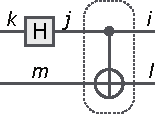
\includegraphics{cnot}
\end{center}
The \CNOT{} and Hadamard gates are defined as
\begin{align}
\CNOT &= \sum_{ab} \ketbra{a, a \oplus b}{a,b}, \quad \\
\label{eqn:hadamard}
\H &= \frac{1}{\sqrt{2}} \sum_{ab} (-1)^{ab} \ketbra{a}{b},
\end{align}
where the addition in the \CNOT{} is modulo~2.\marginnote{Addition modulo 2: $1\oplus 1 = 0\oplus 0 = 0$, \; $1\oplus 0 = 0\oplus 1 = 1$ (see Appendix \ref{sec:Boolean}).} The reader should verify that acting on the quantum state~$\ket{00}$ the above circuit yields the Bell state
$\frac{1}{\sqrt{2}}(\ket{00}+\ket{11})$, and acting on~$\ket{11}$ it yields the singlet state
$\frac{1}{\sqrt{2}}(\ket{01}-\ket{10})$.
\end{example}


\begin{example} [\COPY{} and \XOR{} tensors: cover art] \label{ex:circuits-2}
One can view the \CNOT{} gate itself as a contraction of two order-three tensors (see \S~\ref{sec:btn} for complete details):
\begin{center}
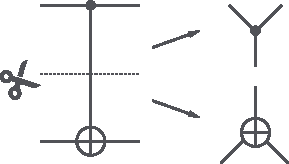
\includegraphics{cnot-tensors}
\end{center}
The top tensor ($\bullet$ with three legs) is called the \COPY{} tensor.
It equals unity when all the indices are assigned the same value ($0$ or $1$), and vanishes otherwise:


\begin{center}
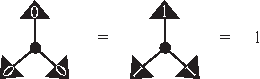
\includegraphics{delta-basis}
\end{center}
Hence, \COPY{} acts to copy the binary inputs $0$ and~$1$:
\begin{subequations}
\begin{align}
        \COPY{} \ket{0} &= \ket{0}\ket{0},\\
        \COPY{} \ket{1} &= \ket{1}\ket{1}.
\end{align}
\end{subequations}

The bottom tensor ($\oplus$ with three legs) is called the parity or \XOR{} tensor.
It equals unity when the index assignment contains an even number of $1$s, and vanishes otherwise:

\begin{center}
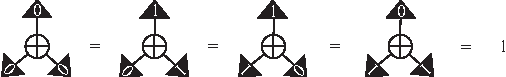
\includegraphics{xor-basis}
\end{center}

The \XOR{} and \COPY{} tensors are related via the Hadamard gate \cite{CD, redgreen} as
\be
\label{eq:copy-vs-xor}
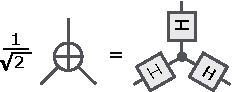
\includegraphics{copy-vs-xor1}
\ee
where the scalars are often omitted when working in the so called, scalar gauge.  Thus one can think of \XOR{} as being a (scaled) copy operation in another basis:
\begin{subequations}
\begin{align}
        \frac{1}{\sqrt{2}}\XOR{} \ket{+} &= \ket{+}\ket{+},\label{eqn:xcopy}\\
        \frac{1}{\sqrt{2}}\XOR{} \ket{-} &= \ket{-}\ket{-},\label{eqn:xcopy2}
\end{align}
\end{subequations}
where $\ket{+} := \H\ket{0}$ and $\ket{-} := \H\ket{1}$. In terms of components,
\begin{subequations}
\begin{align}
\COPY{}\indices{^{ij}_k}
%= 1 - (i + j + k)+ i j + i k + j k
&= (1-i)(1-j)(1-k)+ijk,\\
\XOR{}\indices{^{qr}_s} &= 1-(q+r+s)+2(qr+qs+sr)-4qrs.
\end{align}
\end{subequations}
 
The CNOT gate is now obtained as the tensor contraction
\begin{equation}\label{eqn:cnot}
\sum_m \COPY{}\indices{^{qm}_{i}} \: \XOR{}\indices{^r_{mj}} = \CNOT{}\indices{^{qr}_{ij}}.
\end{equation}

The \COPY{} and \XOR{} tensors will be explored further in later examples and have many convenient properties~\cite{redgreen, BB11,DBCJ11,B17} which will be explained in \S~\ref{sec:btn}.
\end{example} 



\begin{example}[Quantum circuits for cups and epsilon states]\label{ex:state-prep}
The quantum circuit from Example~\ref{ex:circuits-1} is typically used to generate entangled qubit pairs.  
For instance, acting on the state~$\ket{00}$ yields the familiar Bell state---as a tensor network, this is equal to a normalized cup.
Here we also show the mathematical relationship the \XOR{} and \COPY{} tensors have with the cup
($\ket{+}:=\H\ket{0} = \frac{1}{\sqrt{2}}(\ket{0}+\ket{1})$):
\be \label{cnot-bell-states}
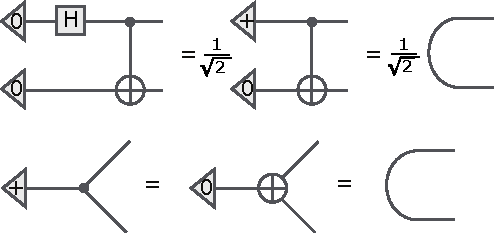
\includegraphics{cups-cnot1}
\ee
Similarly, one can use the circuit~\eqref{eq:bell-circuit} to
generate the epsilon state.
Let us denote the Pauli matrices by $X:=\ket{0}\bra{1}+\ket{1}\bra{0}$, $Y:=-i\ket{0}\bra{1}+i\ket{1}\bra{0}$ and $Z:=\ket{0}\bra{0}-\ket{1}\bra{1}$. 
The $Z$~gate commutes with the \COPY{} tensor, and the $X$ or NOT gate commutes with \XOR{}.
Commuting those tensors to the right hand side,
allows us to apply~\eqref{cnot-bell-states}.  Making use of the Pauli algebra identity $ZX=iY$, one recovers the epsilon state:
\be
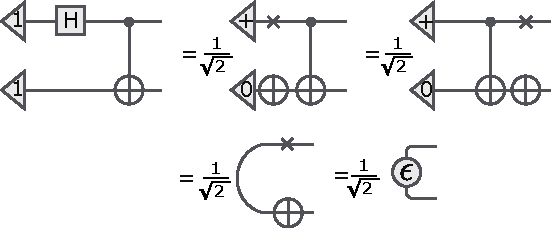
\includegraphics{epsilon-cnot1}
\ee
\end{example}





\begin{remark}[Graphical tensor calculus \cite{Penrose}]
 While many of the examples we have considered so far are simplistic, in practice tensor networks contain an increasing number of tensors, making it difficult to form expressions using (inherently one-dimensional) equations.  The two-dimensional diagrammatic depiction of tensor networks can simplify such expressions, reduce calculations and often depict internal structure that can lend insight into physical phenomena.  
\end{remark}

Equational identities will also be cast into diagrammatic form.  For example, if $\Gamma$ is totally
symmetric in any arm or leg exchange, then we could adopt the convention to draw it as a circle (b).  The tensor in (c) illustrates the equation $A^{b}_{~deg}B^{ac}_{~~f}$.  
\begin{center}
 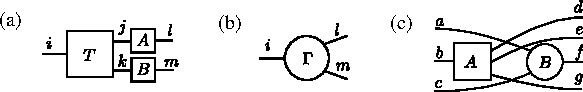
\includegraphics[width=14\xxxscale]{tensors-contraction}
\end{center}

\begin{remark}[Graphical Trace]
 The trace in the graphical calculus is given by connecting wires to close loops \cite{Penrose}.
Diagram (a) below represents the trace~$A\indices{^i_i}$.
Diagram (b) represents the trace~$B\indices{^{iq}_{iq}}$.
\begin{center}
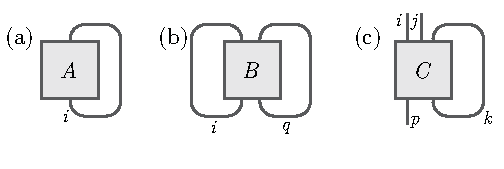
\includegraphics{trace}
\end{center}
Partial trace means contracting only some of the outputs with their
corresponding inputs, such as with the tensor $C\indices{^{ijk}_{pk}}$ shown in diagram (c).
\end{remark}

% \be 
% \psi_{\7 B}(x_1, x_2, \ldots, x_n) = \sum_{x_1, x_2, \ldots, x_n} f(x_1, x_2, \ldots, x_n)\ket{x_1, x_2, \ldots, x_n} \bydef \sum f(\textbf{x})\ket{\textbf{x}} 
% \ee 
% where $f$ takes only binary values, $0$ or $1$, resulting in a wide class of highly correlated quantum states. Here and elsewhere $\textbf{x}$ is defined as $x_1, x_2, \ldots, x_n$.  

% \out{actually they're not used at all, nor are boolean tensors}
\begin{example}[Partial trace]\label{ex:partial-trace}
The following is an early rewrite representing entangled pairs due to Penrose \cite{Penrose67}.
\begin{center}
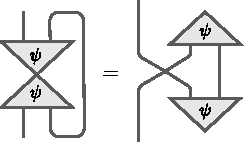
\includegraphics{trace-1}
\end{center}
The diagram on the left represents the partial trace of $\ketbra{\psi}{\psi}$ over the second subsystem.
Readers can prove that this equality follows by interpreting the bent wires as cups and caps, and the crossing wires as \swap{}s.
\end{example}

\begin{example}[Partial trace of Bell states]
 Continuing on from Example \ref{ex:partial-trace}, if we choose $\ket{\psi} = \ket{\cup}$, i.e.~$\ket{\psi}$ is an unnormalized Bell state, we obtain the following. (Compare the following to the diagrams used to model quantum information in the presence of closed timelike curves \cite{Lloyd_2011}.)
\begin{center}
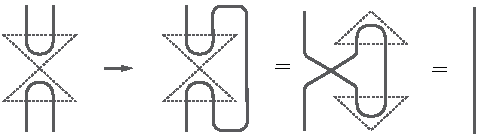
\includegraphics{trace-2}
\end{center}
%The first equality on the left (2nd and 3rd diagram) appears in \cite{road}. 
\end{example}

In general, a quantum state on $n$-spins is a single tensor (such as a box or triangle) with $n$ protruding legs.  Several methods exist to factor such states into elementary building blocks.  For example, it has been shown that the tensor network for each quantum state in the Boolean class of states arises in turn from the classical decomposition of $f$ into fundamental gates.  This is made precise by Theorem \ref{theorem:btns}.  

\begin{remark}[Notation]
We use $\7B$ to denote the Boolean field (this often appears in the literature as $\7F_2$ or as $\7Z_2$), given by an element of the set $\{0,1\}$.  Numbers in $\7B^n$ are then $n$-long Boolean bit strings.  Here and elsewhere, bold font $\textbf{x}$ is shorthand for bit strings $x_1, x_2, \ldots, x_n$.  
\end{remark}

\marginnote{{\it A tensor network representing a Boolean quantum state is determined from the classical network description of the corresponding function}---Theorem \ref{theorem:btns} in \S~\ref{part:count}.}

\begin{definition}[The class of Boolean quantum states --- covered in detail in \S~\ref{sec:btn}]
 Let 
 \be 
 f:\7 B^n \rightarrow \7B ,
 \ee 
 be any switching function.  Then 
 \be 
 \psi_{\7 B} = \sum_{\x}f(\x) \ket{\x},% \ket{}
 \ee 
 is an arbitrary representative in the class of Boolean states.  In this fashion, every Boolean function save the constant zero function, gives rise to a quantum state.  Conversely, every quantum state written in a local basis with amplitude coefficients taking binary values in $\{0,1\}$ gives rise to a Boolean function.  This defines the so called, class of Boolean quantum states (explored in detail in \S~\ref{sec:btn} and \ref{part:count}.
\end{definition}

We will establish the following as Theorem \ref{theorem:btns} in \S~\ref{part:count}: \\

\noindent {\it A tensor network representing a Boolean quantum state is determined from the classical network description of the corresponding function. } \\

\noindent This can be proven by letting each classical gate act on a linear space and from changing the composition of functions, to the contraction of tensors. 






\begin{remark}[Terminology: Boolean tensor networks]\label{remark:boolean}
Boolean tensor networks are in wide use today, but the name ``Boolean tensor network'' is not.  We adopt this terminology in this book however, as part of our presentation which relates these tensors to classical logic gates and networks.  
\end{remark}


\begin{remark}[Quantum Lego blocks: Boolean Tensor Networks]
An example of a Boolean tensor is the \AND-tensor studied in \cite{CTNS}.  This tensor stores the truth table for the local \AND{} function as a superposition.  
\be
\wedge_{ijk} = \sum_{x,y=0,1}\ket{x,y}\ket{x\wedge y} = (\ket{00}+\ket{01}+\ket{10})\ket{0} + \ket{11}\ket{1}.
\ee 
Under Penrose wire-duality, if we bend a wire to raise the index labeled $k$ we arrive at  
 \begin{equation}\label{eqn:AND-map}
 \wedge_{ij}^{~~k}=(\ket{00}+\ket{01}+\ket{10})\bra{0} + \ket{11}\bra{1}.
 \end{equation}
\end{remark}

 
% \begin{remark}[Lower bound on Entanglement Entropy]
%  Explain here.  
% \end{remark}
\begin{remark}[Tensor juxtaposition]
When two or more disconnected tensors appear in the same diagram they are multiplied
together using the tensor product.
In quantum physics notation, they would have a tensor
product sign~$\otimes$ between them.
In the abstract index notation the tensor product sign is omitted.

Tensors can be freely moved past each other.  This is sometimes called planar deformation or rubber sheet topology.
\begin{center}
 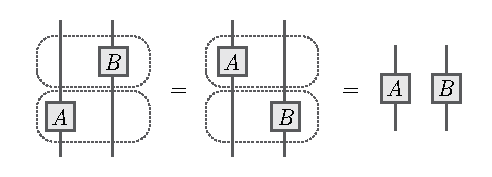
\includegraphics{bifunctorality}
\end{center}
From the diagram above, using equations we have 
\begin{equation}
 (\I\otimes B)(A\otimes \I) = A\otimes B = (A\otimes \I)(\I\otimes B),
\end{equation}
where we make use of the wire also playing the role of the identity tensor~$\I$---detailed in \S~\ref{sec:Bwires}.
As we shall soon see, wires
are allowed to cross tensor symbols and other wires,
as long as the wire endpoints are not changed.
This is one reason why tensor diagrams are often
simpler to deal with
than their algebraic counterparts.
\begin{center}
   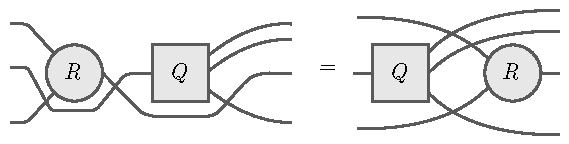
\includegraphics{tensor-01}  
\end{center}

In the diagram above we did not label the wires, since
it is an arbitrary assignment. If we did, we could for example denote it as
$Q\indices{^{deg}_{b}}R\indices{^{f}_{ac}}$.
\end{remark}







\section{Penrose Wire Bending Duality}\label{sec:Bwires}
\paragraph{Bending and exchanging wires.}  Let us consider $n$ Hilbert spaces $\2H^{\otimes n}$.  These spaces are essentially equivalent to each other.  We will then consider the \swap{} operator which exchanges the position of two Hilbert spaces in a composite system, moreover it will exchange the $i$th space with the $i+1$th space, for $1\leq i \leq n-1$.  This generates the permutation group with order that divides $n!$, with the generators given diagrammatically as in (a) 
\begin{center}
 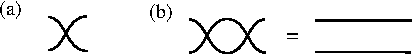
\includegraphics[width=8\xxxscale]{symmetric-map}
\end{center}
where (b) shows that (a) is self inverse. The operator is unitary, and (a) may be written as the tensor
$$
\swap^{ij}_{~~kl}=\delta^i_{~k}\delta^j_{~l},
$$ 
or expanded in the computational basis as 
$$
\swap = \sum_{ij} \ketbra{ij}{ji}.
$$
It also has a well-known implementation in terms of three CNOT gates as  
\begin{center}
    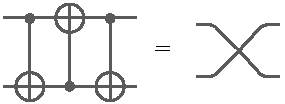
\includegraphics{cnot-swap}
\end{center}


\begin{example}[\swap{} on two Hilbert spaces]
Let $\2 
X$ and $\2 Y$ be complex Hilbert spaces of dimensions $d_1$ and $d_2$ respectively, then the SWAP operation is the map
\be 
\begin{aligned}
\swap{}: \XY &\rightarrow \YX\\
\swap{}: \ket{x}\otimes\ket{y}&\mapsto \ket{y}\otimes\ket{x},
\end{aligned}
\ee
for all $ \ket{x}\in \2 X,\ket{y}\in\2 Y$.

Given any two orthonormal basis 
$$
\{\ket{x_i}: i=0,\hdots, d_1-1\}
$$
and 
$$
\{\ket{y_j}: j=0,\hdots, d_2-1 \}
$$
for $\2 X$ and $\2 Y$ respectively, we can give an explicit construction for the \swap{} operation as\marginnote{{\it Repeated indices to be summed can share the same color in wire diagrams \cite{2011arXiv1111.6950W}.}}
\begin{equation}
\swap{} =  \sum_{i_1=0}^{d_1-1}\sum_{j_2=0}^{d_2-1}\ketbra{y_j}{x_i}\otimes\ketbra{x_i}{y_j}.
\label{eqn:swap}
\end{equation}

The \swap{} operation is represented graphically by two crossing wires as shown:
% FIGURE -  Swap 
\begin{center}
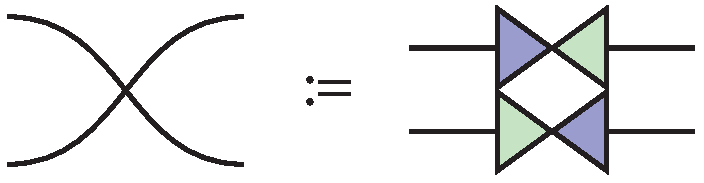
\includegraphics[width=0.35\textwidth]{fig13} 
\label{fig:swap}
\end{center}
The basis decomposition in~\eqref{eqn:swap} is then an application of the resolution of the identity to each wire.
\end{example}

We will now consider the transformation of raising or lowering an index.  One can raise an index and then lower this index or vice versa, which amounts essentially to the net effect of doing nothing at all.  This is captured diagrammatically by the so called, \textit{snake} or \textit{zig-zag equation}, as
\begin{center}
 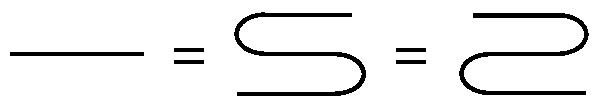
\includegraphics[width=.65\textwidth]{fig11}
\end{center}
together with its vertical reflection across the page.  The snake or zig-zag equation in diagrammatic form dates back at least to Penrose \cite{Penrose}.  Given a basis makes a duality between flipping a bra to a ket, that is, raising or lowering an index, precise.  In tensor index notation, it is given simply by $\delta_{ji}\delta^{ik} = \delta_j^{~k}$.  


 % WIRE BENDING
The mathematical rules of tensor network theory assert that the wires of tensors may be manipulated, with each manipulation corresponding to a specific contraction or transformation.

\begin{myfullpage}  
\begin{definition}
 Transposition of 1st-order vectors and dual-vectors, and 2nd-order linear operators is represented by a \emph{bending} of a tensors wires as follows:
\be
\begin{tabular}{c|c|c}
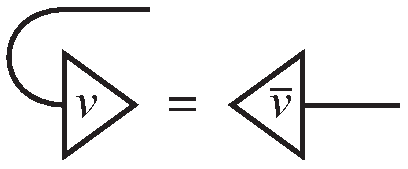
\includegraphics[height=3.5em]{fig3a} \quad\quad&\quad\quad
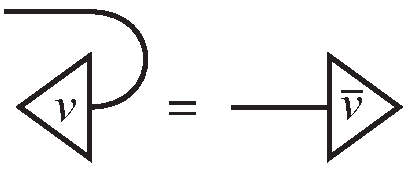
\includegraphics[height=3.5em]{fig3b} \quad\quad&\quad\quad
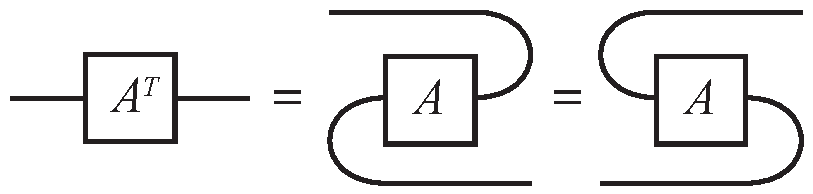
\includegraphics[height=3.5em]{fig3c} \\~\\
\footnotesize{(a) Vector transposition:} \quad&\quad
\footnotesize{(b) Dual-vector transposition:} \quad&\quad
\footnotesize{(c) Linear operator transposition}\\~\\
\footnotesize{$\ket{v}^T = \bra{\overline{v}}$} \quad&\quad
\footnotesize{$\bra{v}^T=\ket{\overline{v}}$} \quad&\quad
\end{tabular}
\label{fig:transpose}
\ee

Complex conjugation of a tensor's coefficients however is depicted by a bar over the tensor label in the diagram: 
 \be
\begin{tabular}{c|c|c}
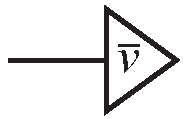
\includegraphics[height=3em]{fig4a} \quad&\quad
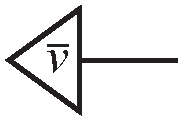
\includegraphics[height=3em]{fig4b} \quad&\quad
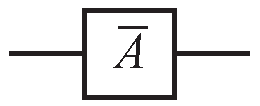
\includegraphics[height=3em]{fig4c} \\
\footnotesize{(a) Complex conjugation of $\ket{v}$} \quad&\quad
\footnotesize{(b) Complex conjugation of $\bra{v}$} \quad&\quad
\footnotesize{(c) Complex conjugation of $A$}
\end{tabular}
\label{fig:conj}
\ee

We stress that under this convention a vector $\ket{v}=\sum_i v_i \ket{i}$ and its hermitian conjugate dual-vector $\bra{v}=\sum_i \overline{v}_i\bra{i}$ are represented as shown in Figure~\ref{sfig}a and~\ref{sfig}b respectively.
\end{definition}
\end{myfullpage}

% \begin{fullpage}
% \begin{example}
%  We may represent the transformation of a vector to its dual vector, or the hermitian conjugation of a linear operator as the combination of these two operations:
% % FIGURE - ADJOINT
% \be
% \begin{tabular}{c|c|c}
% 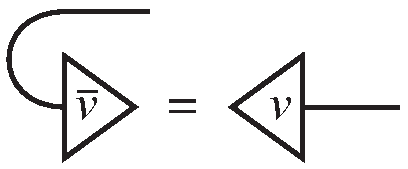
\includegraphics[height=3.5em]{fig5a} \quad&\quad
% 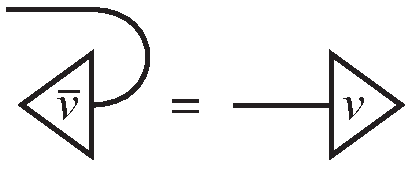
\includegraphics[height=3.5em]{fig5b} \quad&\quad
% 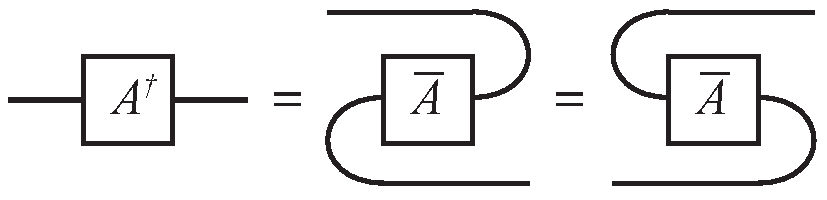
\includegraphics[height=3.5em]{fig5c} \\
% \footnotesize{(a) Hermitian conjugation} \quad&\quad
% \footnotesize{(b) Hermitian conjugation} \quad&\quad
% \footnotesize{(c) Hermitian Conjugation of an operator $A$}\\
% \footnotesize{of a vector : $\ket{v}^\dagger=\bra{v}$} \quad&\quad
% \footnotesize{of a dual-vector : $\bra{v}^\dagger=\ket{v}$} \quad&\quad
% \end{tabular}
% \label{fig:adjoint}
% \ee
% We stress that under this convention a vector $\ket{v}=\sum_i v_i \ket{i}$ and its hermitian conjugate dual-vector $\bra{v}=\sum_i \overline{v}_i\bra{i}$ are represented as shown in Fig.~\ref{sfig:ket} and~\ref{sfig:bra} respectively.
% \end{example}
% \end{fullpage}

 \noindent For explicit examples of writing down the equational form of a tensor diagram refer to the proofs in \S~\ref{app:tensor1}.
\paragraph{Equivalence class.}  In further detail, we will consider the class of operations formed from bending tensor wires forwards or backwards using cups and caps, as well as exchanging wires using \swap{}.  We can conceptualize this class of transforms acting on a tensor as, amounting essentially, to matrix reshapes. From the snake equation, action with a cup or cap is invertible and \swap{} is self inverse.  This means that, all possible configurations of a tensors legs using these operations are equivalent, when the equivalence is taken up to Penrose duality.    

\begin{lemma}[Cardinality of index manipulations]
 Given a tensor $T^{ij}$ with fixed labels $i,j$ we can use cups and caps to arrive at 
\be 
 T^{ij}, ~ T^{i}_{~j} , ~ T_{ij}, ~ T_{i}^{~j},
\ee 
the \swap{} operation reorders $i$ and $j$ and then the cups and caps yield 
\be 
 T^{ji}, ~  T^{j}_{~i} , ~  T_{ji}, ~ T_{j}^{~i}.
\ee 
In general, for a tensor with a total of $n$ indices, each index can be up or down, yielding $2^n$ possibilities.  The symmetry group formed by \swap{} is of order $n!$ and acts to arrange the $n$ legs of a tensor, yielding 
\be
n!\cdot 2^n
\ee 
different ways to reorder the indices of a tensor, provided we distinguish $T_{i}^{~j}$ and $T^{j}_{~i}$ etc.  
\end{lemma}

\begin{remark}[Ordering operators by numbers of inputs and outputs]\label{remark:ordering-index}
In the previous remark, we considered $T_{i}^{~j}$ (b) and $T^{j}_{~i}$ (a) etc., as distinct.  For all practical purposes, they are not however.  This is shown as follows.  
 \begin{center}
 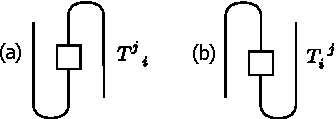
\includegraphics[width=7\xxxscale]{penrose-duality-II}
\end{center}
This shows an awkward property of standard Dirac notation.  Both (a) and (b) represent the same map, but when we write this in a basis, one of them will require us to write $\bra{i}\otimes\ket{j}$.  

With this in mind, we note that the tensor $T_{ij}$ which was considered in the last section actually has 6 unique reshapes, as two of the reshapes are diagrammatically equivalent.  
 \begin{center}
 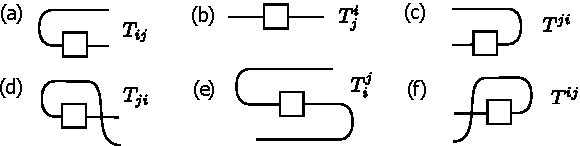
\includegraphics[width=10\xxxscale]{penrose-duality}
\end{center}
\end{remark}
% For instance, 
% \begin{center}
%  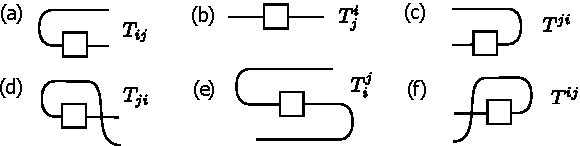
\includegraphics[width=12\xxxscale]{penrose-duality}
% \end{center}
% illustrates the possible ways to reshape an order-two tensor.  If the operator is given by say $T$, then (a) represents $\sum_{ij} T^i_j\ket{i}\bra{j}$ (top) with the transpose $\sum_{ij} T^i_j\ket{j}\bra{i}$ found from wire exchange (bottom), (b) $\sum_{ij} T^i_j\bra{j}\bra{i}$, (c) $\sum_{ij} T^i_j\bra{i}\bra{j}$, (d) $\sum_{ij} T^i_j\ket{i}\ket{j}$ and (e) $\sum_{ij} T^i_j\ket{j}\ket{i}$.  These tensors are all isomorphic as (i) the bending of wires can be undone via the snake equation, and (ii) the reordering of spaces can be undone, since the swap operation squares to identity.  %In (c) and (e) the equals sign down the page illustrates that the swap operation commutes with the cups and caps.  

The duality is well know, but we have not seen mention of the order.  We call this the \emph{natural tensor symmetry class}.  In Theorem \ref{theorem:symmetry-class} we are going to count (i) the number of possible ways a tensor can have its wires bent, either forward or backwards using the cups and caps, in conjunction with (ii) the number of ways a tensor can have its arms and/or legs exchanged.    
\begin{theorem}[Natural tensor symmetry class]
\label{theorem:symmetry-class}
The arms and legs of a tensor $\Gamma^{ij\cdots k}_{qr\cdots s}$ with $m$ input arms $(ij\cdots k)$ and $n$ output legs $(qr\cdots s)$, can be rearranged in  
\be 
(n+m+1)! 
\ee
different ways.
\begin{proof}
Exercise.  
% Bend all the wires to one side and note that you can pull any one or any other back, act before this or after this with the permutation group generators, but actually, it is easy to see that this commutes, so we only have to count the order of each and then multiply the result.  
\end{proof}
\end{theorem}


\section{Bending Density Operator Wires}

We will now apply the natural tensor symmetry class counted in Theorem \ref{theorem:symmetry-class} to the analysis of the quantum states arising from bending wires on density operators.  These states are found by bending all the wires of a tensor representing a density operator to the same side, as follows.  
\begin{center}
 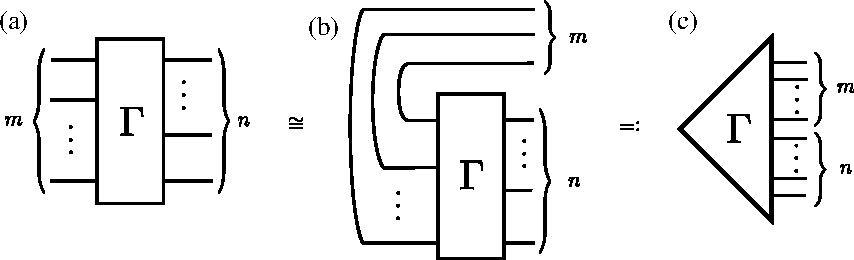
\includegraphics[width=10\xxxscale]{eqv-class}
\end{center} 
For the case of a density map, $m=n$.  

We will first compare the idea of a matrix basis with that of a vector space basis both for an inner product space.  We will use these concepts to study symmetries of 
density operators.  In fact, 
\begin{remark}[Injection from Density Operators to States --- Theorem \ref{theorem:injection}]
 We will soon prove that the existence of an injective map sending each n-party density matrix $\rho$ to a quantum state.  The map is found by bending wires.  The resulting state is naturally equivalent under SWAP to $2n!$ states, by Theorem \ref{theorem:symmetry-class}.    
\end{remark}
The process is invertible.  However, every quantum state does not always give rise to a $\rho$ under wire duality.  The purpose of the present section is to make these statements precise.  

\subsubsection*{Matrix basis}
We expand $d$-dimensional operators using a matrix basis $\{A_i\}$,
which is orthonormal with respect to the \emph{Hilbert-Schmidt} inner product, defined as
\be 
\langle A_i,A_j\rangle :=
\frac{1}{d}\Tr(A_i^\dagger A_j)=\delta_{ij}.
\ee 
The product $A_iA_j$ is given in (a)
\begin{center}
 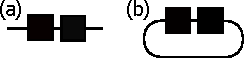
\includegraphics[width=5\xxxscale]{trace-norm1}
\end{center} 
and the trace inner product in (b).
Here and elsewhere in this work, all scale factors in the diagrams are omitted graphically, but we note that care must be taken when one is summing over diagrams. 


\begin{example}[Pauli matrix basis] 
A nascent example of a matrix basis with the described properties is the Pauli matrices on qubits.  Any operator of type $\C^2\rightarrow\C^2$ can be written in terms of the Pauli matrices as 
\be 
a \I + \vec{p} \cdot \vec{\sigma} = a \I + bX+cY+dZ,
\ee
for $a,b,c,d\in \C$.  Note that this provides a decomposition into a symmetric subspace 
\be
\1S= \text{span}\{\I, X, Z\},
\ee 
and an antisymmetric subspace $\1A=\text{span}\{Y\}$.  This symmetry is exhibited by $\rho = \rho^\top\in\1S$ and antisymmetry as $\rho = -\rho^\top\in\1A$.  Diagrammatically, transposition is done by twisting a map (see (a) or (b) in Remark \ref{remark:ordering-index}) \cite{Kassel}.  
\end{example}

\subsubsection*{Vector basis} For a vector space basis $\{a_i\}$ in $\C^2\otimes \C^2$ we use the typical inner product where
\be
\langle a_i,a_j\rangle = \delta_{ij},
\ee 
which is given diagrammatically as in (b).  (a) Follows from the diagrammatic SVD, and the black square is intended to depict a not necessarily unitary, or for that matter invertible, map.   
\begin{center}
 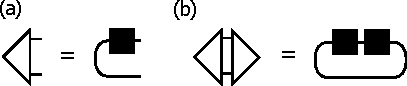
\includegraphics[width=10\xxxscale]{state-basis1-2}
\end{center} 

\begin{example}[Bell vector basis] 
An example of a vector basis is the Bell basis on qubits.  Any vector
in $\C^2\otimes\C^2$ can be written in terms of this basis as (see
Table~\ref{table:pauli-vs-bell})
\be 
\psi(a,b,c,d) = a \Phi^+ + b \Phi^- + c \Psi^+ + d \Psi^-,
\ee
for $a,b,c,d\in \C$.  This partitions the space into a symmetric subspace 
\be 
\1s=\Span\{ \Phi^+, \Phi^- ,\Psi^+ \},
\ee 
and an antisymmetric subspace $\1a=\Span\{\Psi^-\}$.  This symmetry is illustrated by $\psi(i,j) = \psi(j,i)\in\1s$ and antisymmetry as $\psi(i,j) = -\psi(j,i)\in\1a$.  Diagrammatically, this amounts to letting the swap gate act on both output wires, which serves to exchange them.  
\end{example}


\subsubsection*{Comparison} 
We note that in the diagrammatic language, the Bell vector basis and the Pauli matrix basis become essentially equivalent as they are related by bending wires.  
In particular, we note that they have identical form as the operator basis norm and the inner product of vectors.  These are both, up to a scale factor, identical in the graphical language.  To illustrate our point, we present the following table.  

\begin{table}[h!]
\centering
\begin{tabular}{ccc}
\hline
$\C^2\rightarrow\C^2$ &  & $\C^2\otimes\C^2$\\
\hline 
$\I$ & $\cong$ & $\Phi^+ = \ket{00}+\ket{11}$\\
$\sigma^x$ & $\cong$ & $\Psi^+ = \ket{01}+\ket{10}$\\
$\sigma^y$ & $\cong$ & $\Psi^- = i(\ket{01}-\ket{10})$\\
$\sigma^z$ & $\cong$ & $\Phi^- = \ket{00}-\ket{11}$\\
\hline
\end{tabular}
\caption{Mapping between Pauli matrices and Bell states.
\label{table:pauli-vs-bell}
}
\end{table}
Table~\ref{table:pauli-vs-bell} illustrates the specific mapping between Pauli matrices and Bell states.  For example, the second row represents 
\begin{center}
 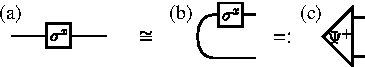
\includegraphics[width=10\xxxscale]{pauli-vs-bell}
\end{center} 
where (a) is the $\sigma^x$ matrix.  By bending a wire, we arrive at (b) which is identically equal to the bell state $\Psi^+$ in (c).  
% I have already defined this elsewhere, but for didactic purposes I think it is well-suited to repeat this.


\subsubsection*{Density operators vs pure states.}  We are in a position to carry out an analysis of the class of states found by bending the wires of a density operator all to the same side.  
We first consider the expansion of a density operator into the so called Hilbert-Schmidt basis of Pauli operators.  
We let 
\be 
P_n = \{\I, X, Y, Z\}^{\otimes n},
\ee 
be the set of all $n$ letter words, formed from the alphabet of Pauli
matrices, with $\otimes$ as the concatenation operator.  The span of
$P_n$ forms a Hermitian operator basis as each element is invariant
under the $\dagger$.  We can expand any density operator $\rho$ in
terms of this basis as 
\be 
\rho = \sum a^{ijk\cdots l}\sigma_i \sigma_j\sigma_k\cdots \sigma_l,
\ee 
for an $n$-long index $ijk\cdots l$, where each $i,j,k$ etc indexes an
operator in $P_n$.  We can now study the natural embedding of this
operator $\rho$ on ${\C^2}^{\otimes n}\rightarrow {\C^2}^{\otimes n}$ into
$\psi_\rho \in {\C^2}^{\otimes 2n}$.

\begin{theorem}[Injection from density operators to states]
\label{theorem:injection}
Every density operator $\rho$ on $\2H^{\otimes n} \rightarrow
\2H^{\otimes n}$ gives rise to a state $\psi_\rho$ in $\2H^{\otimes  2n}$.
This state has $2n!$ natural symmetries induced by swap.

\begin{proof}
Each density operator is dual to a state by bending wires.  We will express this starting with the density operator
\be 
\rho = \sum a^{ijk\cdots l}\sigma_i \sigma_j\sigma_k\cdots \sigma_l,
\ee
and writing it as 
\be 
\psi_\rho = \sum a^{ijk\cdots l}\Psi_i\otimes \Psi_j\otimes \Psi_k\otimes \cdots \otimes \Psi_l,
\ee
where $\Psi_m \cong \sigma_m$ per bending a wire on each $\sigma_m$, and arriving at the state $\psi_\rho$.  This results in the quantum state $\psi_\rho$.  Note that 
there are a number of choices of ordering when bending the wires.  In addition, these wires can be arbitrarily ordered after bending 
to still form an essentially equivalent state.  In fact, one can act with the symmetry group on the open wires, to arrive at the natural symmetry class with the same order as the permutation group.  This scenario is depicted below.   
\end{proof}
\end{theorem}

\begin{example}[Injection from density operators to states]
We can illustrate the idea behind Theorem \ref{theorem:injection} in the following figure.  (a) depicts density operator $\rho^i_{~j}$ and (b) $\rho_{ij}$ its state dual. 
 \begin{center}
 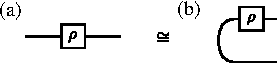
\includegraphics[width=8\xxxscale]{rho-to-state-2}
\end{center}
\end{example}


\begin{remark}[From states to operators by Penrose wire duality]
While every density operator gives rise to a
quantum state, the converse is not necessarily true.
The condition $\rho = \rho^\dagger$ corresponds to $a^{ijk\cdots l} \in \R$
which limits the possible states.
For the case of qubits, a quantum state has
$2(2^n-1)$ real degrees of freedom in general, whereas the states
arising under Theorem \ref{theorem:injection} have $2^n-1$ real degrees of freedom.
% TODO positivity of \rho
\end{remark}


\begin{remark}[In general wire bending is not purification] 
 Let 
\be 
\rho = \frac{1}{2}\I + \sigma.A = \frac{1}{2}\I + a X + b Y + c Z,
\ee 
be the arbitrary state of a qubit.  Then by Theorem \ref{theorem:injection}, 
\be
\psi_\rho = (1+c)\ket{00} + (a+bi)\ket{01} + (a-bi)\ket{10} + (1-c)\ket{11}, 
\ee
is the natural state-dual to $\rho$ with norm $\braket{\psi_\rho}{\psi_\rho} = 2(a^2+b^2+c^2)$. However, we note that 
Theorem \ref{theorem:injection} does not in general provide a purification of $\rho$.  
\end{remark}


\begin{remark}[Symmetric density operators vs symmetric states]
A symmetric single qubit density operator necessarily has $bY=0$ and so gives rise to a symmetric two qubit state with real valued coefficients parametrized by two real degrees of freedom, $\psi_\rho(a, 0, c)$.  Diagrammatically, a symmetric two-party state is invariant under exchange of its legs (a) whereas a symmetric density operator is invariant under exchange of its arms and legs (e.g.\ transpose), (b).  
\begin{center}
 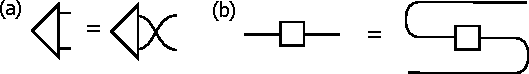
\includegraphics[width=10\xxxscale]{2-party-symmetric-states1}
\end{center}
\end{remark}

% \begin{remark}[Injection from unitary maps to quantum states]
%  We have defined an the injection from density operators into quantum states and derived some of its key properties.  Results of a similar nature can be worked out for unitary maps.  
% SAY something of interest here, like these are all locc to bell states!  
% \end{remark}


% note that a density operator is dagger but not always transpose symmetric.  what does this mean for the states?  

\subsection{Bipartite Matrix Operations}
\label{sec:bipartite}

Bipartite matrices are used in several representations of CP-maps, and manipulations of these matrices will be important in the following discussion.
\begin{definition}
Consider two complex Hilbert spaces $\2 X$, and $\2 Y$ with dimensions $d_x$ and $d_y$ respectively. The bipartite matrices we are interested in are then $d^2_x\times d^2_y$ matrices $M\in {\mathcal L}(\2X\otimes\2Y)$ which we can represent as 4th-order tensors with tensor components
\begin{equation}
M_{m\mu,n\nu}:=\bra{m, \mu}M\ket{n,\nu}
\end{equation} 
where $m,n \in \{0,...,d_x-1\}$, $\mu,\nu \in \{0,...,d_y-1\}$ and $\ket{n,\nu}:=\ket{n}\otimes\ket{\nu}\in \2X\otimes\2Y$ is the tensor product of the standard bases for $\2 X$ and $\2 Y$.
\end{definition}

 Graphically this is given by
% FIGURE - BIPARTITE TENSOR

\begin{center}
  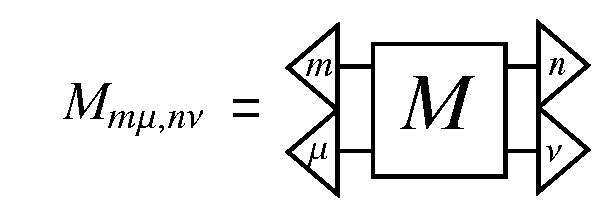
\includegraphics[height=5em]{fig14a}
 \label{fig:bipartite-m-4}  
\end{center}


We can also express the matrix $M$ as a 2nd-order tensor in terms of the standard basis $\{\ket{\alpha} : \alpha = 0,\hdots,D-1\}$ for $\2X\otimes\2Y$ where $D=d_x d_y$. In this case $M$ has tensor components
\begin{equation}
M_{\alpha\beta}=\bra{\alpha}M\ket{\beta}
\end{equation}
This is represented graphically as
% FIGURE - BIPARTITE TENSOR
\begin{center}
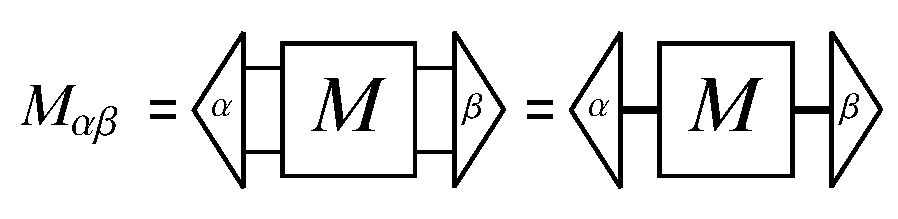
\includegraphics[height=5em]{fig14b}
 \label{fig:bipartite-m-2}
\end{center}

We can specify the equivalence between the tensor components $M_{\alpha\beta}$ and $M_{m\mu,n\nu}$ by making the assignment
\begin{eqnarray}
\alpha &=& d_x m + \mu\\
\beta &=& d_y n +\nu,
\end{eqnarray} 
where $d_y$ is the dimension of the Hilbert space $\2 Y$.

\begin{fullpage}
The bipartite matrix operations which are the most relevant for open quantum systems (see Fig.~\ref{fig:cpreps}) are the \emph{partial trace over $\2 X$}  ($\Tr_{\2 X}$) (and $\Tr_{\2 Y}$ over $\2 Y$), \emph{transposition} ($T$), \emph{bipartite}-\SWAP{} ($S$), \emph{col-reshuffling} ($R_c$), and \emph{row-reshuffling} ($R_r$). The corresponding graphical manipulations are:
% FIGURE - BIPARTITE TENSOR
\begin{center}
 \begin{tabular}{cccccc}
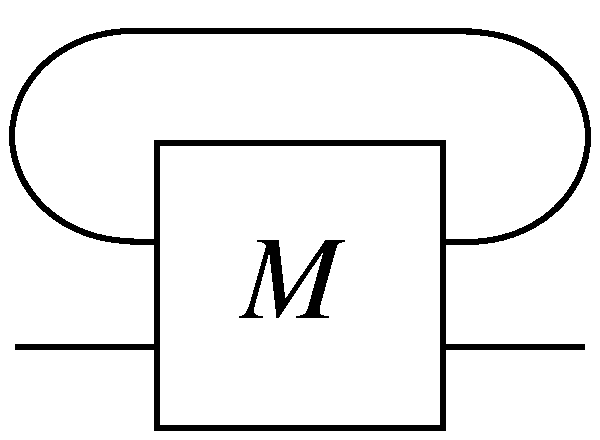
\includegraphics[width=0.1\textwidth]{fig15a}	\quad&\quad
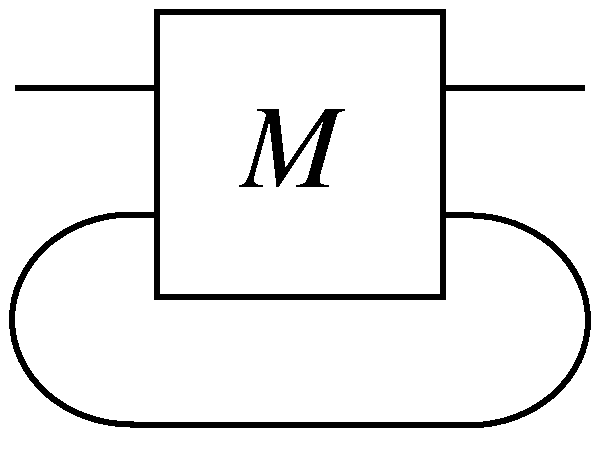
\includegraphics[width=0.1\textwidth]{fig15b}	\quad&\quad
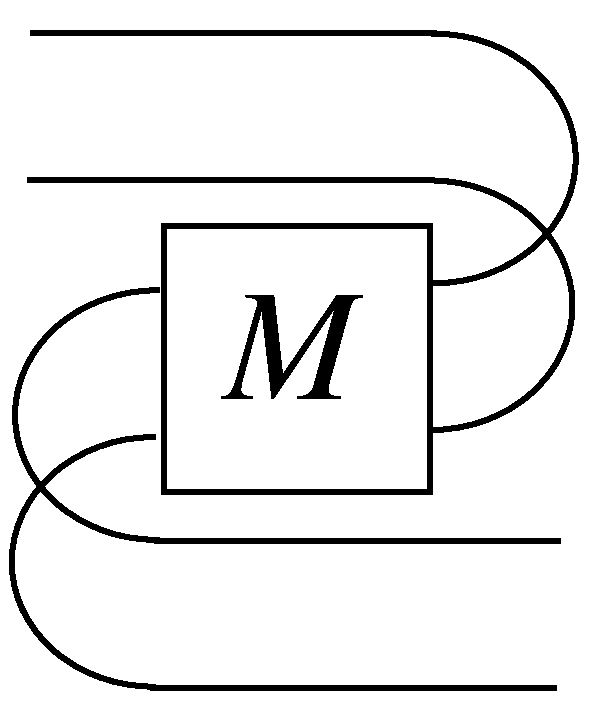
\includegraphics[width=0.1\textwidth]{fig15c}	\quad&\quad
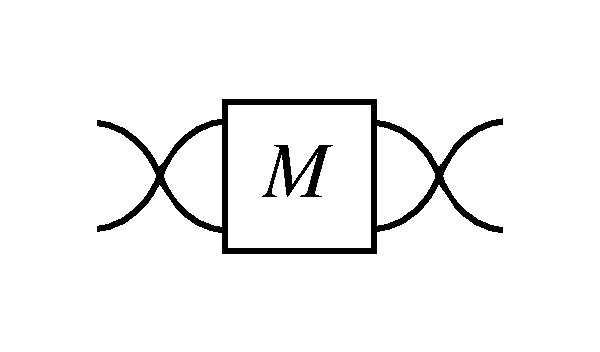
\includegraphics[width=0.13\textwidth,trim=1.5cm 1.5cm 1.5cm 1.5cm,clip]{fig15d}	\quad&\quad
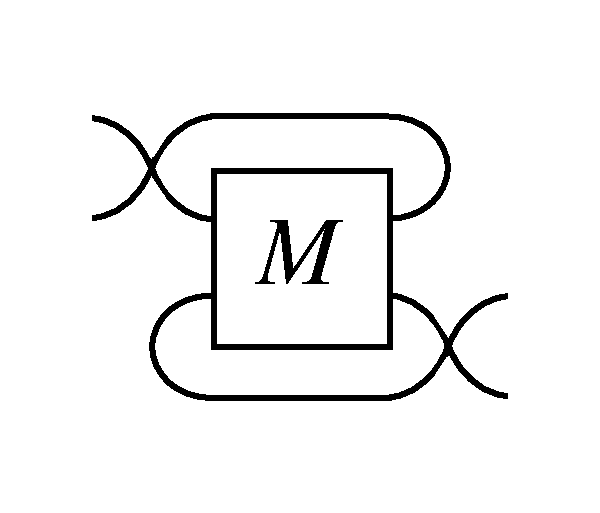
\includegraphics[width=0.1\textwidth,trim=1.5cm 1.5cm 1.5cm 1.5cm,clip]{fig15e}	\quad&\quad
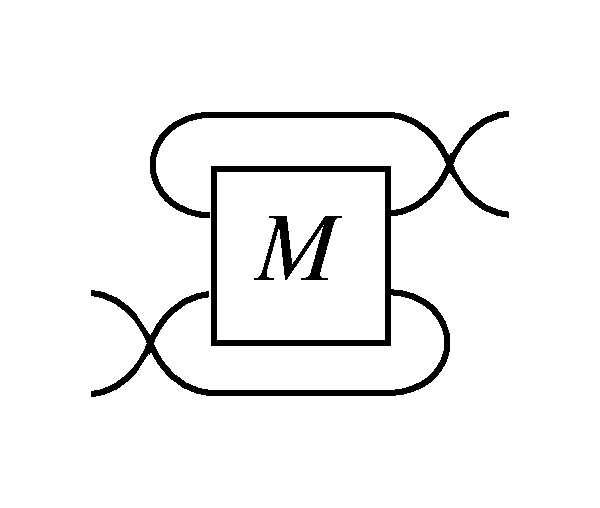
\includegraphics[width=0.1\textwidth,trim=1.5cm 1.5cm 1.5cm 1.5cm,clip]{fig15f}	\\
\footnotesize{(a) Partial Trace} \quad&\quad
\footnotesize{(b) Partial Trace} \quad&\quad
\footnotesize{(c) Transpose} \quad&\quad
\footnotesize{(d) Bipartite-Swap} \quad&\quad
\footnotesize{(e) Row-Reshuffle} \quad&\quad
\footnotesize{(f) Col-Reshuffle} 
\\
\footnotesize{$\Tr_{\2 X}[M]$} \quad&\quad
\footnotesize{$\Tr_{\2 Y}[M]$} \quad&\quad
\footnotesize{$M^T$} \quad&\quad
\footnotesize{$M^S$} \quad&\quad
\footnotesize{$M^{R_r}$} \quad&\quad
\footnotesize{$M^{R_c}$} 
 \end{tabular}
 \label{fig:bipartite}
\end{center}
 In terms of the tensor components of $M$ these operations are respectively given by:
\begin{center}
\begin{tabular}{lll}
Partial trace over $\2X$
\quad&\quad	$\Tr_{\2 X}: {\mathcal L}(\2X\otimes\2Y)\rightarrow {\mathcal L}(\2Y),$ 
\quad&\quad	$M_{m\mu,n\nu} \mapsto \sum_{m} M_{m\mu,m\nu}$
\\
Partial trace over $\2Y$
\quad&\quad	$\Tr_{\2 Y}: {\mathcal L}(\2X\otimes\2Y)\rightarrow {\mathcal L}(\2X)$
\quad&\quad	$M_{m\mu,n\nu} \mapsto \sum_{\mu} M_{m\mu,n\mu}$
\\
Tranpose
\quad&\quad	$T: {\mathcal L}(\2X\otimes\2Y)\rightarrow {\mathcal L}(\2X\otimes\2Y),$ 
\quad&\quad	$M_{m\mu,n\nu} \mapsto M_{n\nu,m\mu}$
\\
Bipartite-\SWAP{}
\quad&\quad	$S: {\mathcal L}(\2X\otimes\2Y)\rightarrow {\mathcal L}(\2Y\otimes\2X),$ 
\quad&\quad	$M_{m\mu,n\nu} \mapsto M_{\mu m, \nu n}$
\\
Row-reshuffling
\quad&\quad	$R_r: {\mathcal L}(\2X\otimes\2Y)\rightarrow {\mathcal L}(\2Y\otimes\2Y,\2X\otimes\2X),$ 
\quad&\quad	$M_{m\mu,n\nu} \mapsto M_{m, n , \mu, \nu} $
\\
Col-reshuffling
\quad&\quad	$R_c: {\mathcal L}(\2X\otimes\2Y)\rightarrow {\mathcal L}(\2X\otimes\2X,\2Y\otimes\2Y),$ 
\quad&\quad	$M_{m\mu,n\nu} \mapsto M_{\nu \mu, n m}$
\end{tabular}
\end{center}
%
Note that we will generally use reshuffling $R$ to refer to col-reshuffling $R_c$. Similarly we can represent the partial transpose operation by only transposing the wires for $\2X$ (or $\2Y$), and the partial-\SWAP{} operations by only swapping the left (or right) wires of $M$.\\
\end{fullpage}

%%%%%%%%%%%%%%%%%%%%%%%%%%%%%%%%%%%%%%%%%%%%%%%%%%%%%%%%%%%%
\subsection{Vectorization of Matrices}
\label{sec:vec}
We now recall the concept of \emph{vectorization} which is a reshaping operation, transforming a $(m\times n)$-matrix into a $(1\times mn)$-vector~\cite{Horn1985}. This is necessary for the description of open quantum systems in the superoperator formalism, which we will consider in \S~\ref{sec:sop}.
\begin{definition}
Vectorization can be done with using one of two standard conventions: \emph{column-stacking} (col-vec) or \emph{row-stacking} (row-vec). Consider two complex Hilbert spaces $\2 X\cong \C^m, \2 Y\cong \C^n$, and linear operators  $A\in {\mathcal L}(\2X,\2Y)$ from $\2 X$ to $\2 Y$. Column and row vectorization are the mappings
\begin{eqnarray}
\mbox{col-vec: } {\mathcal L}(\2X,\2Y)&\rightarrow& \XY: \,\, A\mapsto\dket{A}_c\\
\mbox{row-vec: } {\mathcal L}(\2X,\2Y)&\rightarrow& \YX: \,\,A\mapsto\dket{A}_r
\end{eqnarray} 
respectively, where the operation col(row)-vec when applied to a matrix, outputs a vector with the columns (rows) of the matrix stacked on top of each other. 
\end{definition}



\begin{myfullpage}
\begin{illexample}
Graphical representations for the row-vec and col-vec operations are found from bending a wire to the left either clockwise or counterclockwise respectively:
% FIGURE - VEC DEF
\begin{center}
\begin{tabular}{c|c}
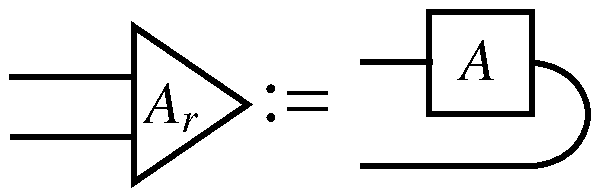
\includegraphics[height=3.5em]{fig16a} 
\quad\quad&\quad\quad
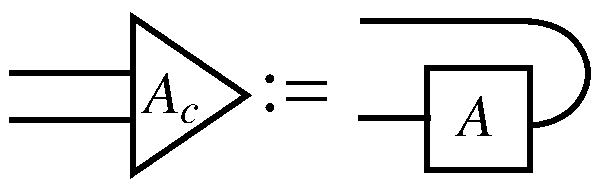
\includegraphics[height=3.5em]{fig16b} 
\\
\footnotesize{(a) Row-vec} &
\footnotesize{(b) Col-vec}
\end{tabular}
 \label{fig:vectorization}
\end{center}
Vectorized matrices in the col-vec and row-vec conventions are naturally equivalent under wire exchange (the \SWAP{} operation)
% FIGURE - COL ROW SWAP
\begin{center}
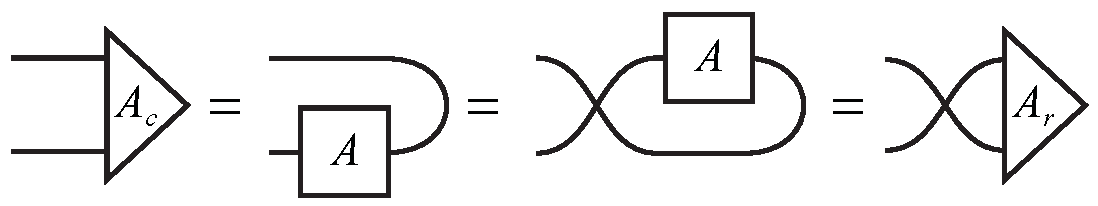
\includegraphics[width=.55\textwidth]{fig17} \label{fig:col-to-row}    
\end{center}


In particular we can see that the unnormalized Bell-state $\ket{\Phi^+}\in\2X\otimes\2X$ is in fact the vectorized identity operator $\I\in {\mathcal L}(\2X)$
\begin{equation}
\ket{\Phi^+} = \dket{\I}_r = \dket{\I}_c.
\end{equation}
\end{illexample}
\end{myfullpage}

\begin{definition}
We may also define a vectorization operation with respect to an arbitrary operator basis for ${\mathcal L}(\2X,\2Y)$. Let $\2 X\cong\C^{d_x}, \2 Y\cong \C^{d_y}$, and $\2Z \cong \C^D$ where $D=d_x d_y$. Vectorization with respect to an orthonormal operator basis $\{\sigma_\alpha:\alpha=0,...,D-1\}$ for ${\mathcal L}(\2X,\2Y)$ is given by
\begin{equation}
	\sigma\mbox{-vec: }{\mathcal L}(\2X,\2Y)\rightarrow \2Z :\,\,A\mapsto \dket{A}_\sigma.
\end{equation}
This operation extracts the coefficients of the basis elements returning the vector  
\begin{equation}
	\label{eqn:trace-rep}
	\dket{A}_\sigma := \sum_{\alpha=0}^{D-1} \Tr[\sigma^\dagger_\alpha A] \ket{\alpha}
\end{equation}
where $\{\ket{\alpha}: \alpha=0,...,D-1\}$ is the standard basis for $\2Z\cong\C^D$. This is depicted in our graphical calculus as 
% FIGURE - BASIS VEC
\begin{center}
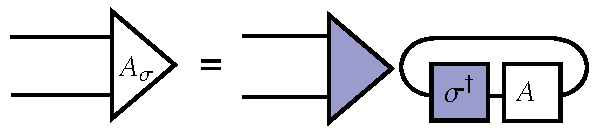
\includegraphics[width=.65\textwidth]{fig18} \label{fig:basis-vectorization}  
\end{center}
\begin{remark}
  To distinguish between these different conventions we use the notation $\dket{A}_x$ to denote the vectorization of a matrix $A$, were the subscript $x=c,r,\sigma$ labels which convention we use; either $c$ for col-vec, $r$ for row-vec, or $\sigma$ for an arbitrary operator basis.
\end{remark}
 
For the case $\2 X\cong\2 Y\cong \C^d$, we can define row-vec and col-vec in terms of~\eqref{eqn:trace-rep} by taking our basis to be the elementary matrix basis $\{ E_{i,j}=\ketbra{i}{j} : i,j=0,...,d^2-1\}$, and making the assignment $\alpha=di+j$ and $\alpha=i+dj$ respectively. Hence we have
\begin{eqnarray}
\dket{A}_r &:=& \sum_{i,j=0}^{d-1} A_{ij}\, \ket{i}\otimes\ket{j}	\label{eqn:rowvec}\\ 
\dket{A}_c &:=& \sum_{i,j=0}^{d-1} A_{ij}\, \ket{j}\otimes\ket{i}	\label{eqn:colvec}.
\end{eqnarray} 
\end{definition}

\begin{example}
Using the definition of the unnormalized Bell-state $\ket{\Phi^+}$ and summing over $i$ and $j$ one can rewrite~\eqref{eqn:rowvec} and \eqref{eqn:colvec} as
\begin{eqnarray}
\dket{A}_r &=& (A \otimes \I) \ket{\Phi^+}\label{eqn:row-vec}\\
\dket{A}_c &=& (\I \otimes A) \ket{\Phi^+}\label{eqn:col-vec}
\end{eqnarray}
which are the equational versions of our graphical definition of row and col vectorization shown in \eqref{fig:vectorization}.
 \end{example}
 
When working in the superoperator formalism for open quantum systems, it is sometimes convenient to transform between vectorization conventions in different bases. Given two orthonormal operator bases $\{\sigma_\alpha\}$ and $\{\omega_\alpha\}$ for ${\mathcal L}(\2X,\2Y)$, the basis transformation operator 
\begin{equation}
T_{\sigma\rightarrow\omega}: \2Z\rightarrow\2Z: \dket{A}_\sigma\mapsto \dket{A}_\omega
\end{equation} 
transforms vectorized operators in the $\sigma$-vec convention to the $\omega$-vec convention. Graphically this is given by

% FIGURE - VEC BASIS CHANGE
\begin{center}
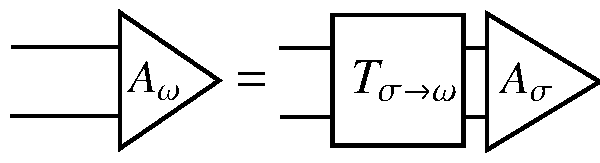
\includegraphics[width=0.5\textwidth]{fig19} \label{fig:vec-basis-change}
 \end{center}
The basis transformation operator $T_{\sigma\rightarrow\omega}$ is given by the equivalent expressions
\begin{equation}
T_{\sigma\rightarrow\omega} 
	= \sum_\alpha \ket{\alpha}\dbra{\omega_\alpha}_\sigma 	
	= \sum_\alpha \dket{\sigma_\alpha}_\omega\bra{\alpha} 	\label{eqn:vec-change},
\end{equation}
and the corresponding graphical representations are: 
% FIGURE
\begin{center}
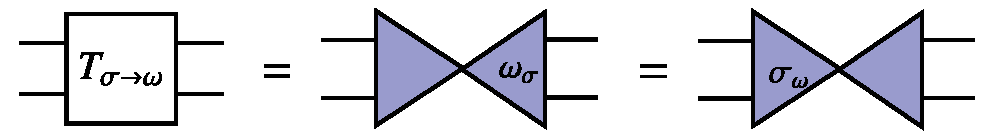
\includegraphics[width=0.8\textwidth]{fig20alt}\label{fig:basis-change-op}
\end{center}
%The proofs of Eq.~\eqref{eqn:vec-change-1} and \eqref{eqn:vec-change-2} are found in Appendix~\ref{app:vec-proofs}.

As in \cite{2011arXiv1111.6950W}, we tend to use the col-vec convention by default, and drop the vectorization label subscripts unless referring to a general $\sigma$-basis. The main transformation we will be interested in is then from col-vec to another arbitrary orthononormal operator basis $\{\sigma_\alpha\}$. Tensor networks for the change of basis $T_{c\rightarrow\sigma}$ and its inverse $T_{\sigma\rightarrow c}$ are
% FIGURE
\begin{center}
 \begin{tabular}{c|c}
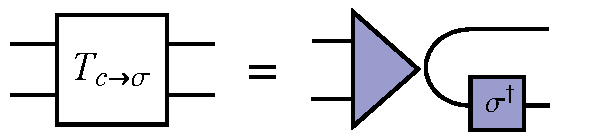
\includegraphics[width=0.45\textwidth]{fig21a}	
\quad\quad&\quad\quad
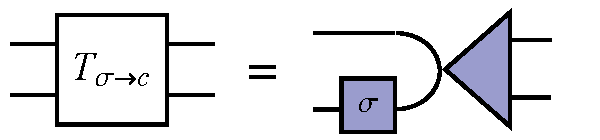
\includegraphics[width=0.45\textwidth]{fig21b}	
\\
\footnotesize{(a) Col-vec to $\sigma$-basis} &
\footnotesize{(b) Row-vec to $\sigma$-basis} 
\end{tabular}
 \label{fig:vec-basis-col}
\end{center}
In the case where one wants to convert to row-vec convention, as previously shown the transformation is given by
\begin{equation}
T_{c\rightarrow r}=T_{r\rightarrow c}= \mbox{SWAP}.
\end{equation}
%TODO Page 23, the figure at the top: (b) is titled as "Row-vec to \sigma-basis".  I guess it should be the inverse of "Col-vec to \sigma-basis", i.e., "\sigma-basis to Col-vec".


One final important result that often arises when dealing with vectorized matrices is Roth's Lemma for the vectorization of the matrix product $ABC$~\cite{Horn1985}.  Given matrices $A,B,C\in {\mathcal L}(\2X)$ we have
\begin{eqnarray}
\dket{ABC} &=& (C^T\otimes A) \dket{B}
\label{eqn:roth}
\end{eqnarray}
The graphical tensor network proof of this lemma is as follows:\mn{The theory of tensor networks leverages one to study the
mathematical structure formed by the composition of processes and states on the same footing.} 
% FIGURE
\begin{center}
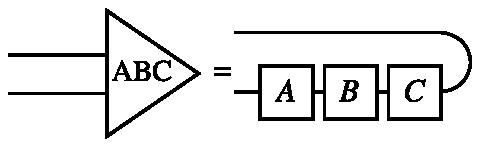
\includegraphics[width=0.45\textwidth]{fig22a}
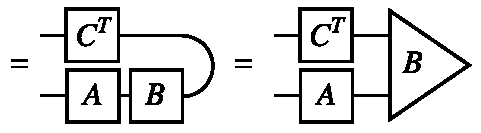
\includegraphics[width=0.45\textwidth]{fig22b}
\label{fig:vecabc}
\end{center}

\section{Worked Examples}
\label{app:tensor1}

We will now prove the consistency of several of the basic tensor networks introduced in Part~\ref{sec:tensor}, and in doing so illustrate how one may use our graphical calculus for diagrammatic reasoning.  

The color summation convention we have presented represents diagrammatic summation over a tensor index by coloring the appropriate tensors in the diagram. In this convention summation over a Kronecker delta, $\sum_{i,j}\delta_{ij}=\sum_{i,j} \braket{i}{j}$, is as shown:
% FIGURE - DELTA
\be
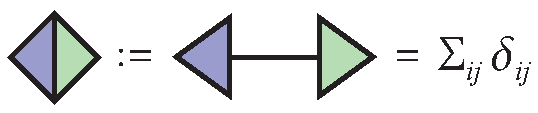
\includegraphics[width=0.3\textwidth]{fig48}
\label{fig:delta-sum}
\ee
This expression is used in several of the following proofs.


We begin with the proof of the trace of an operator $A$:
% FIGURE -  TRACE PROOF
\be
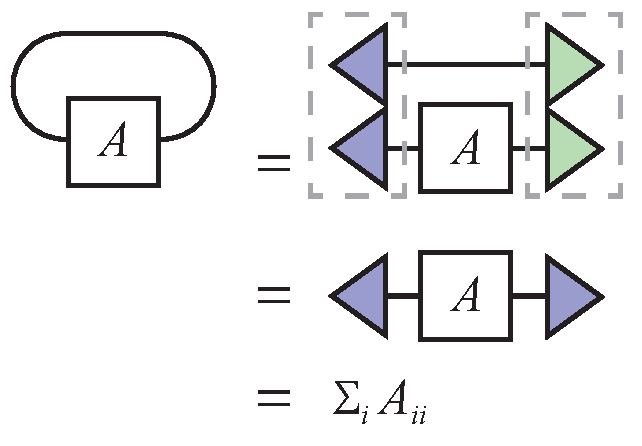
\includegraphics[width=0.3\textwidth]{fig49}
\label{fig:trace-proof}
\ee
 
For illustrative purposes, to prove this algebraically we note that the tensor networks for trace correspond to the algebraic expressions $\bra{\Phi^+}A\otimes\I\ket{\Phi^+}$ and $\bra{\Phi^+}\I\otimes A\ket{\Phi^+}$, and that
\begin{eqnarray}
\bra{\Phi^+}\I\otimes A\ket{\Phi^+}
&=& \sum_{i,j}\braket{i}{j}\bra{i}A\ket{j}
= \sum_{i,j} \delta_{ij} A_{ij}\nonumber\\
&=& \sum_i A_{ii}\\
&=& \Tr[A].\nonumber
\end{eqnarray}
Similarly we get $\bra{\Phi^+}A\otimes\I\ket{\Phi^+}=\Tr[A]$.

To prove the snake equation we will want to move some triangles around.
This is illustrated diagrammatically as
\begin{marginfigure}
\centering
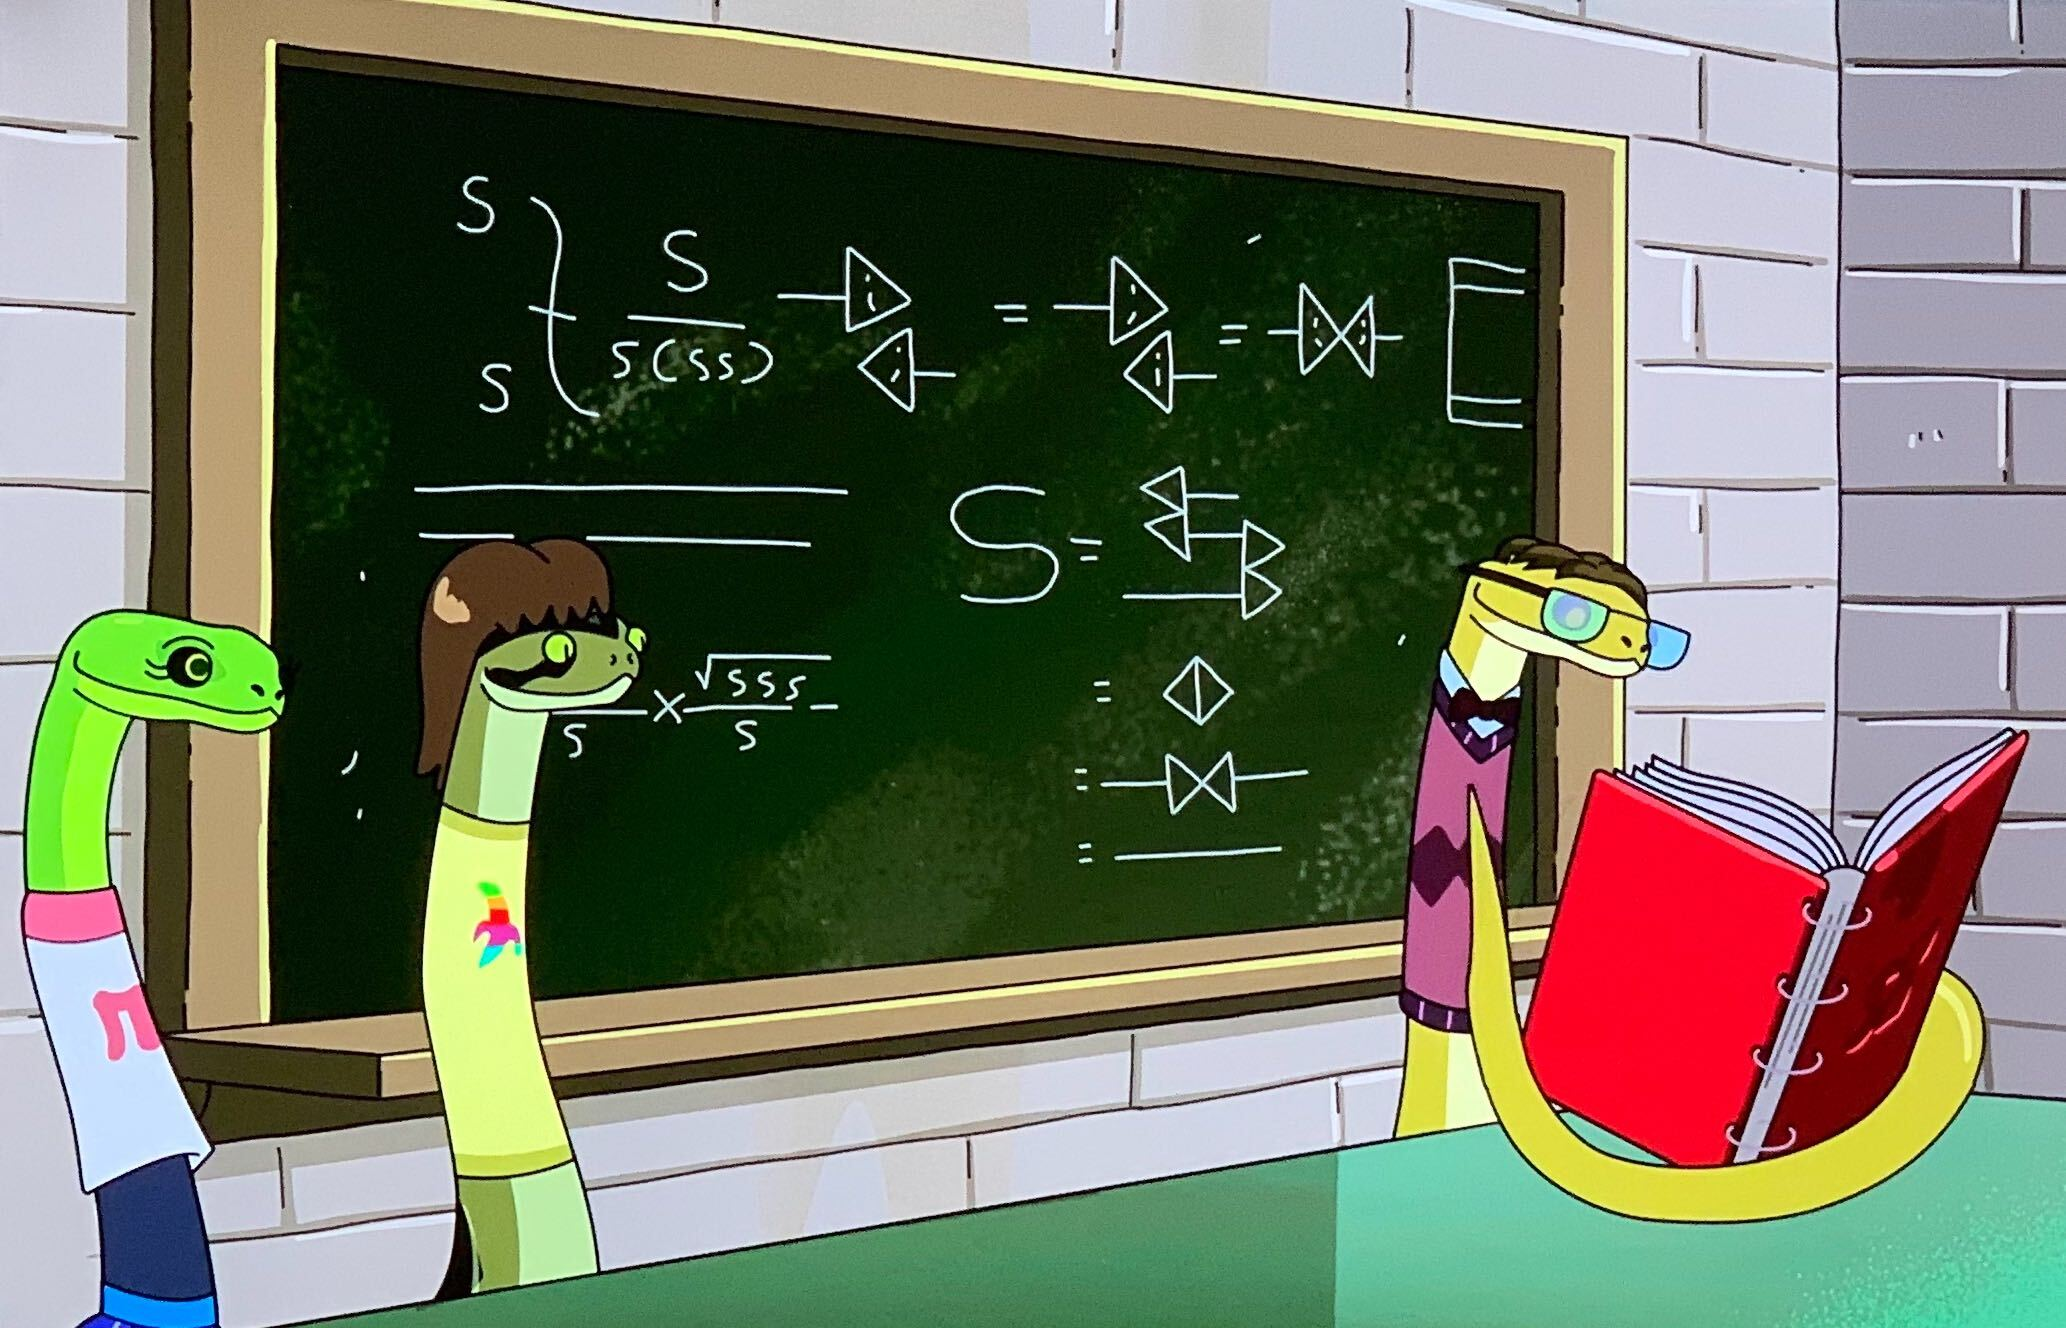
\includegraphics[width=6.0\xxxscale]{SnakeRM.jpg}
\caption{Current Rick and Morty dressed as snakes travel to 1985 and leave a copy of this book at Snake MIT. However, they arrived too late: the snakes have already written equations \eqref{fig:tensor-product-equiv} and \eqref{fig:snake-proof} on their chalkboard, adapted to enable snake-time travel of course.  These equations first appeared in a study I coauthored with Chris Wood and David Corey \cite{Woo+15}. And yes, it was used to create the chalkboard in Snake MIT (Season 4: Episode 5, Rattlestar Ricklactica). In a final plot twist, I actually learned the colour of this very book watching this episode, embroiling all readers in a grandfather-paradox with Rick and Morty.  
Rick tells Morty, ``{\bf That book contains everything they need to create snake time travel}'':  but it's too late.  The snakes have already copied equations \eqref{fig:tensor-product-equiv} and \eqref{fig:snake-proof} to their chalkboard at {\it Snake MIT 1985} in Rick and Morty, Season 4: Episode 5, {\it Rattlestar Ricklactica}. The figure first appeared in joint work with Chirs Wood and David Corey~\cite{2011arXiv1111.6950W}.}
\end{marginfigure}
% FIGURE -  TENSOR EQUIV
\be
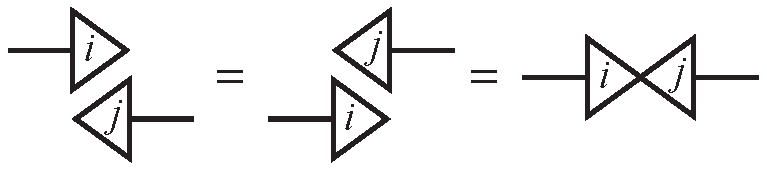
\includegraphics[width=0.4\textwidth]{fig50}
\label{fig:tensor-product-equiv}
 \ee




With this equivalence made, the proof of the snake-equation for the ``S'' bend is given by
% FIGURE -  SNAKE PROOF
\be
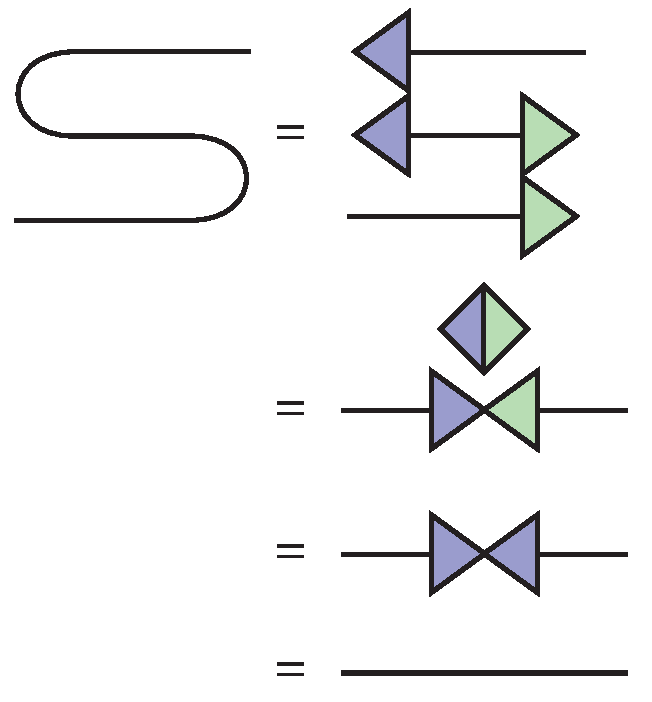
\includegraphics[width=0.3\textwidth]{fig51}
\label{fig:snake-proof}
\ee
The proof for the reflected ``S'' snake-equation follows naturally from the equivalence defined in \eqref{fig:tensor-product-equiv}.

The proof of our tensor network for the transposition of a linear operator $A$ is as follows:
% \begin{marginfigure}
% \centering
% 
\includegraphics[width=5\xxxscale]{SnakeRM2.jpg}
% \caption{The figure first appeared in joint work with Wood and Corey~\cite{2011arXiv1111.6950W} and (at the time when I wrote this) is the first hit for ``snake equation'' using Google image search.}
% \end{marginfigure}
% FIGURE -  TRANSPOSE PROOF 1
\be
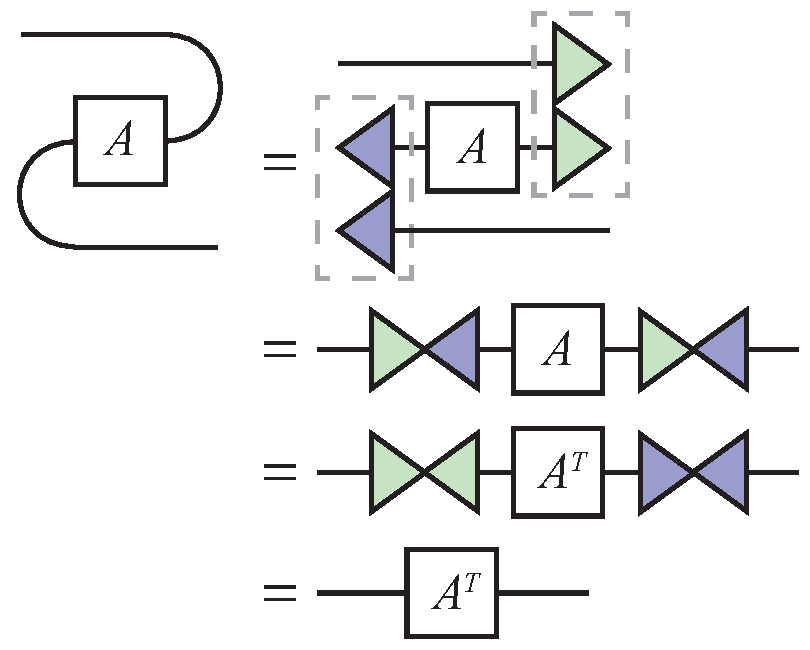
\includegraphics[width=0.35\textwidth]{fig52a}
\label{fig:tensor-transpose-proof-1}
\ee
To prove this algebraically we note that the corresponding algebraic equation for the transposition tensor network is
\begin{eqnarray}
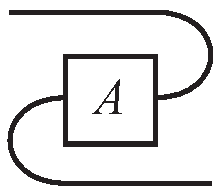
\includegraphics[width=0.09\textwidth]{inline-fig5}&=&\I\otimes\bra{\Phi^+}(\I\otimes A\otimes\I)\ket{\Phi^+}\otimes\I\\
&=& \sum_{i,j} \bra{j}A\ket{i}\ \ket{i}\otimes\bra{j}\\
&=& \sum_{i,j} \bra{j}A\ket{i} \ketbra{i}{j}\\
&=& \sum_{i,j} \bra{i}A^T\ket{j} \ketbra{i}{j}\\
&=& \sum_{i,j} \ketbra{i}{i}A^T\ketbra{j}{j}\\
&=& A^T.
\end{eqnarray}
The proof for transposition by counter-clockwise wire bending follows from the equivalence relation in \eqref{eqn:tensor-product-equiv} and \eqref{fig:tensor-product-equiv}. 

With the tensor network for transposition of an operator proven, the proof of transposition by contracting through a Bell-state $\ket{\Phi^+}$ is then an application of the snake equation as shown:
 % FIGURE -  TRANSPOSE PROOF 2
\be
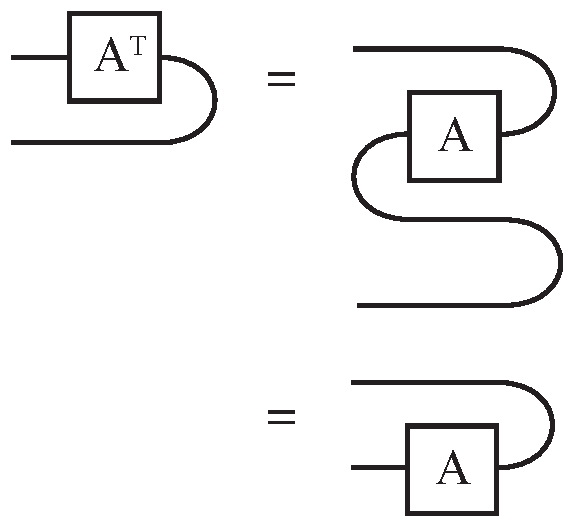
\includegraphics[width=0.3\textwidth]{fig53}
\label{fig:bell-tr-proof}
\ee  
%%%%%%%%%%%%%%%%%%%%%%%%%%%%%%%%%%%%%%%%%%%%%%%%%%


\section{Problems} 

\begin{myexercise}(Bell basis). 
Using the right hand side equations, 
\begin{eqnarray*}
\sigma_0 = \sum \ketbra{a}{a},\qquad \sigma_1 = \sum \ketbra{1-a}{a},
\\
\sigma_2=i\sum (-1)^{a+1} \ketbra{a}{1-a},\qquad \sigma_3 =\sum (-1)^a\ketbra{a}{a}.
\end{eqnarray*}
for $a\in \{0,1\}$. 
Show that 
\begin{equation}
\frac{1}{\sqrt{2}}\left(\sum_{l\in\{0,1\}} \bra{l} \otimes \bra{l} \right) \overline{\sigma_i} \otimes \I = \frac{1}{\sqrt{2}}\sum_{l\in\{0,1\}} (\bra{l}\overline{\sigma_i}) \otimes \bra{l},
\end{equation}
defines the Bell effects (which defines an orthonormal basis in $\mathbb{C}^2\otimes \mathbb{C}^2$). Here $\sigma_i$ indexes the Pauli matrices.\mn{Effects are dual to states.  Also called, costates.}
\end{myexercise}

%%%%%%%%%%%%%%%%%%%%%%%%%%%%%%%%%%%%%%%%%%%
\begin{remark}
Complete the following problems using standard techniques and then compare this to graphical tensor network approach. 
\end{remark}
%%%%%%%%%%%%%%%%%%%
\begin{myexercise}
Suppose $\psi \in \mathbb{C}_2^{\otimes 2}$ and $E>0$ with $E\in \mathcal{L}(\mathbb{C}_2^{\otimes 2})$. Show that 
\begin{equation}
    \bra{\psi}E\otimes \I \ket{\psi}, 
\end{equation}
takes the same values when $\psi$ is any of the four Bell states.
\end{myexercise}

%%%%%%%%%%%%%%%%%%%
\begin{myexercise}[Transpose or Ricochet Trick]
Show that 
\begin{equation}
(M^A\otimes \I^B)\ket{\Phi}^{AB} = (\I^A \otimes (M^\top)^B)\ket{\Phi}^{AB},
\end{equation}
for maximally entangled $\ket{\Phi}^{AB}$ and any matrix $M$. 
\end{myexercise}

%%%%%%%%%%%%%%%%%%%

\begin{myexercise}
Show that the purity $P(\rho^A)$ is equal to 
\begin{equation}
    P(\rho^A) = \Tr\{ (\rho^A\otimes \rho^{A'}) F^{AA'}\},
\end{equation}
where Hilbert space $A$ is isomorphic to $A'$ and $F^{AA'}$ is the swap operator defined on a basis (indexed by $x,y$) as 
\begin{equation}
    F^{AA'}\ket{x}^A\ket{y}^{A'}=\ket{y}^A\ket{x}^{A'}.
\end{equation}
Hint. Establish that 
\begin{equation}
    \Tr\{f(\rho^A)\}= \Tr\{(f(\rho^A)\otimes \I^{A'} )F^{AA'}\},
\end{equation}
for function $f$ of the operators on $A$. 
\end{myexercise}

\section{Further Reading}

Readers should be aware of the high number of quality tutorials covering various aspects of tensor networks available for free download from the arXiv.org preprint server.  Many but not all of these are also published in journals. For those interested in applications to condensed matter, we particularly recommend. \\

\noindent {\bf Hand-waving and Interpretive Dance: An Introductory Course on Tensor Networks} \cite{2016arXiv160303039B}\\
Jacob Bridgeman and Christopher Chubb \\
J.~Phys.~A: Math.~Theor.~50 223001 (2017)
\href{https://arxiv.org/abs/1603.03039}{arXiv:1603.03039}\\

For those interested in the mathematics of string diagrams (category theory), the most accessible introduction covering the foundations of the building blocks presented in this chapter can be found in. \\

\noindent {\bf A Prehistory of n-Categorical Physics} \cite{Baez}\\
John Baez and Aaron Lauda\\
Deep Beauty 13–128, Cambridge University Press (2011) \href{https://arxiv.org/abs/0908.2469}{arXiv:0908.2469} \\

In addition to this work on the categories of tensor networks \cite{Baez}, readers might also find the survey \cite{catQM} of interest.  For a tour of the categories relevant in quantum theory see e.g.~\cite{0198739613} and for a survey of applications see \cite{Coecke2017}. 

Category theory is worth considering as a mathematical framework to describe wire diagrams (including quantum circuits).  Category theory itself is sophisticated enough to present a theorem that essentially proclaims that the diagrams contain {all} relevant information.  Hence one might say that {\it category theory formally rules out the need for category theory}---provided one knows how to manipulate the tensor diagrams. This is formally stated in the following well-known theorem. 

\begin{theorem}[Coherence for categories \cite{Selinger_2010}] A well-formed equation between two morphism terms in the language of categories follows from the axioms of categories if and only if it holds in the graphical language up to isomorphism of diagrams.
\end{theorem}

Hence, readers should be aware that the formal mathematics of tensor networks finds its roots in {\it tensor category theory} (now often renamed {\it dagger categories}). And that the diagrams themselves are proven to contain the relevant information \cite{Selinger_2010}. The topic of modeling the theory of quantum mechanics using categories was explored intensively in the area the authors from \cite{catQM} named, {\it categorical quantum mechanics}---see the book \cite{Coecke2017} for a survey. 

There are two fundamental types of tensor networks in wide use today.  The most common is similar to quantum circuits (which is the topic of this book).  The second is the braided class of tensor networks, used in topological quantum computing.  In terms of active research, recently a class of tensor networks was discovered by Jaffe, Liu and Wozniakowski---the JLW-model---notably, the wires carry charge excitations \cite{Liu2017, Jaffe2016,Jaffe2018}.  The rules in which network components can be moved, merged and manipulated in a graphical form of reasoning take an elegant form with known applications to quantum protocols~\cite{Jaffe2017}.  For instance the relative locations on wires carries precise meaning and changing the ordering modifies a connected network specifically by a complex number.  The type of isotopy discovered in the topological JLW-model provides an alternative means to reason about quantum information, computation and protocols.  Some open problems related to the JLW-model are given in \cite{JaffeLiu2017}.  


\newpage 
\part{Matrix Product States} 

One of the most common uses of tensor networks in quantum information is representing states which belong to small but physically relevant subset of a much larger Hilbert space.  This often includes low-entanglement states. The  backbone of this idea rests on low rank matrix approximations which we will consider in this chapter.  

We will see that if one partitions a network, by cutting it in two, the number of wires that were cut in this process provides an upper bound on the maximum amount of possible entanglement between spins. 
This can be made more precise by considering the (unitarily invariant) entanglement entropy of a bipartite split.  
\begin{equation}\label{eqn:entropy}
E = -\Tr\left(\rho \text{ln} \rho \right) = - \sum_i \lambda_i \text{ln} \lambda_i.
\end{equation}  
Here $\lambda_i$ are the singular values of the reduced density operator of either subsystem.  The quantity is maximized for all $\lambda_i$ equal to the inverse of the dimension of a reduced density matrix. The value of \eqref{eqn:entropy} provides a quantitative measure of correlations.  This will be elaborated as a central concept in what follows.   
\begin{marginfigure}
\centering
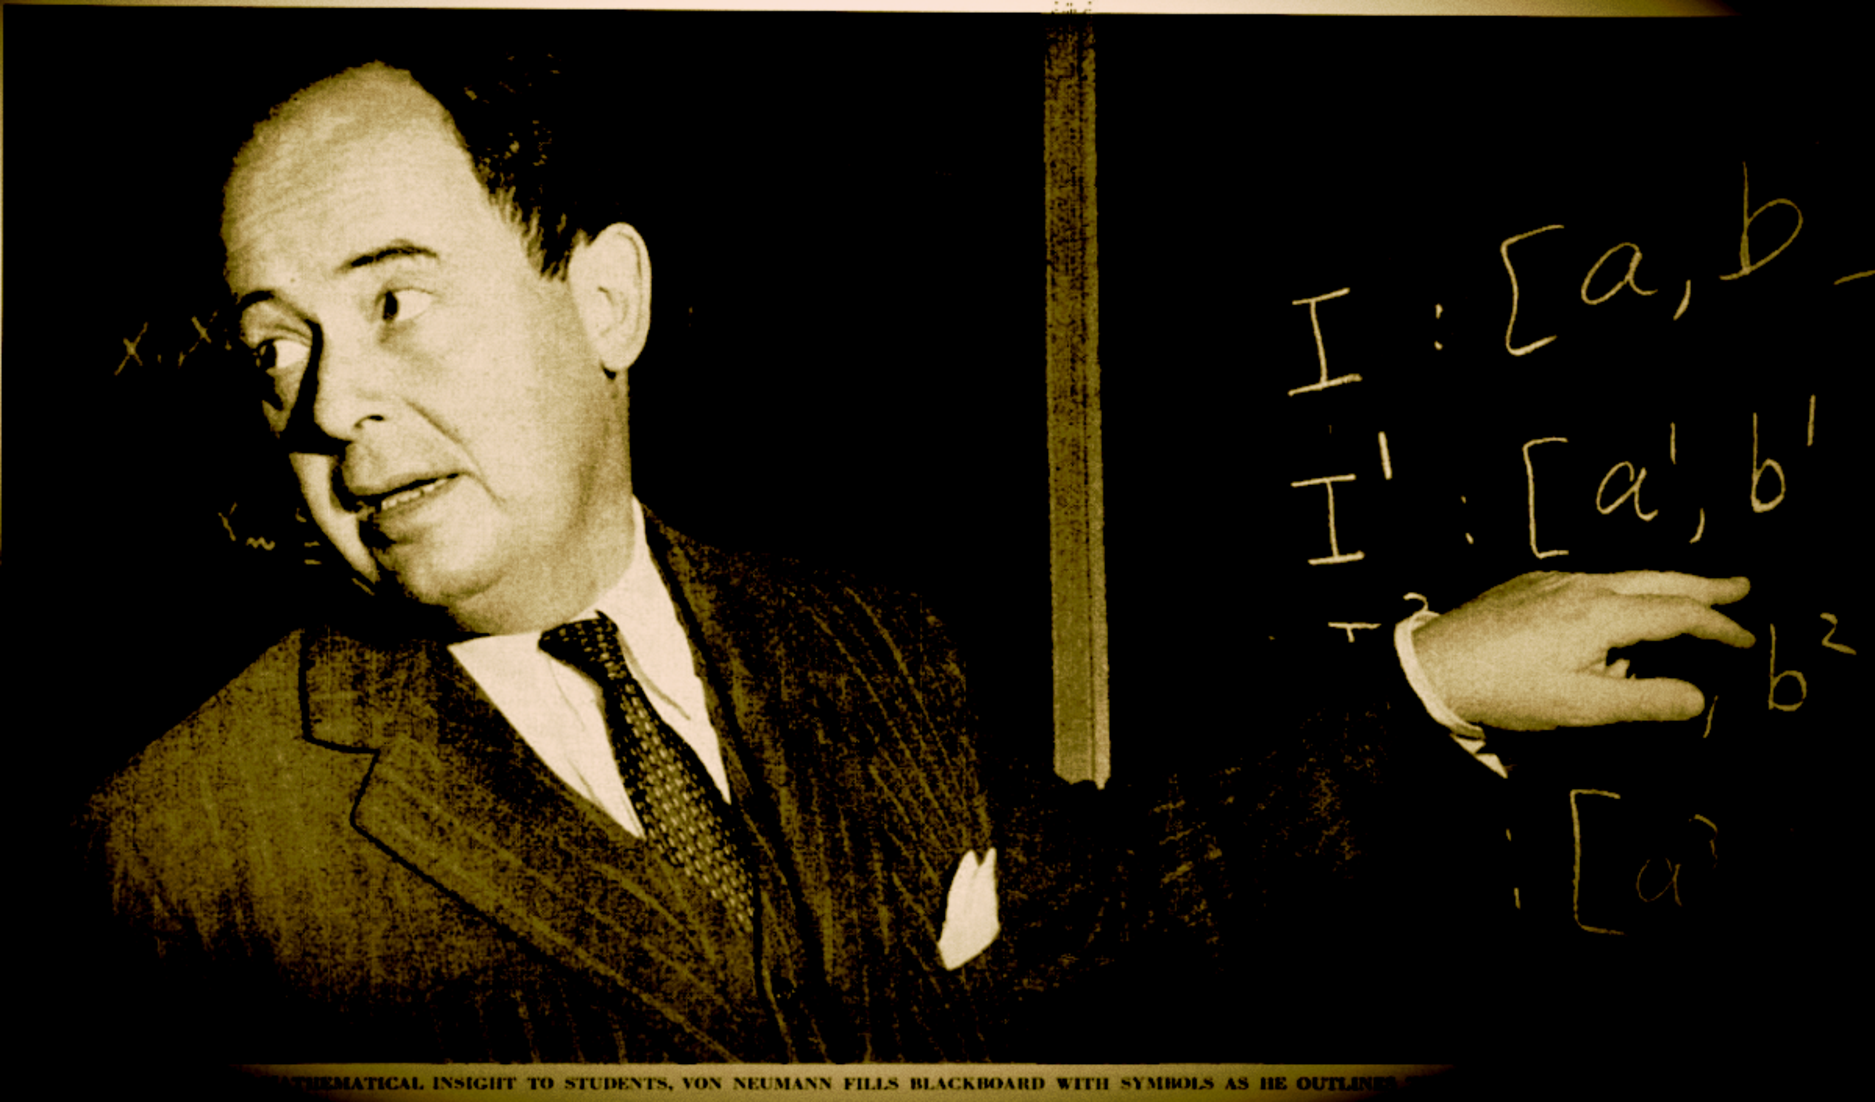
\includegraphics[width=6\xxxscale]{Neumann-Banner}
\caption{``\textit{You should call it entropy, for two reasons. In the first place your uncertainty function has been used in statistical mechanics under that name, so it already has a name. In the second place, and more important, no one really knows what entropy really is, so in a debate you will always have the advantage.}''\\~\\
John von Neumann suggesting to Claude Shannon a name for his new uncertainty function, as quoted in Scientific American {\bf 225}(3) 180, (1971).}
\end{marginfigure}


\section{The Diagrammatic SVD}

In this section, we will introduce a diagrammatic form of the singular
value decomposition (SVD).  It is assumed that the reader has solved Exercise \ref{exercise:svd1} (see also Exercise \ref{exercise:rank1}). 

There are several utilities to our
approach.  The first stems from the fact that the known invariants we
have studied can be simplified by network contraction using the diagrammatic SVD.   
The method factors tensor into well defined building blocks
with simplistic interaction properties: black \COPY-tensors and white
unitary boxes.  We will also consider the iteration of this process, allowing one to arrive at matrix product states (MPS) in terms of our network building blocks. 

An aim of the present work is to consider how graphical depictions of tensors can leverage a better understanding of how certain properties evident in a network are reflected in properties related to a quantum state.  Intuitively one thinks of a connected network as representing a correlated or entangled state.  This chapter will push this idea further.  




% Here we will make use of symmetric tensors as studied in~\cite{BB10}.
% We define a family of tensors as follows: 
% \begin{definition}[Diagonal tensors]
% \label{def:diagonal-tensors}
% An $m$-to-$n$ diagonal tensor $D^{ij\cdots k}_{qr\cdots s}$ where each
% arm and each leg has dimension~$d$ is defined in the standard basis as
% \begin{equation}\label{eqn:diagonal-tensors}
% D^{ij\cdots k}_{qr\cdots s} := \sum_{l=0}^{d-1} a_l \ketbra{\underbrace{l \cdots l}_{n}}{\underbrace{l \cdots l}_{m}},
% \end{equation}
% where $a_l \in \C$.  Tensors in this class are clearly invariant under (i) permutation of their wires, (ii) wire exchange 
% from input to output and (iii) iff each of the components $a_l$ takes only real values, then the tensor is symmetric under the dagger operation. General properties of such tensors, including fusion rules etc. can be found in~\cite{BB10}.
% \end{definition}

\COPY{}-tensors have been studied in the setting of the Penrose
tensor calculus, in work dating back at least to Lafont \cite{boolean03} and explored more recently using an alternative notation in the so called ZX-calculus \cite{CD, redgreen} --- see also \cite{BB11, CTNS}.
Here we apply \COPY{}-tensors in the diagrammatic SVD factorization of quantum states.  The key diagrammatic properties are illustrated as follows and explained in detail in \S~\ref{sec:btn}.  

\begin{definition}[Properties of the \COPY-tensor]\label{def:copy-prop}
The copy property is illustrated in (b).  Here a basis state, or copy point $\ket{x}$ is contracted with the \COPY{}-tensor, which then breaks into two copies of $\ket{x}$. These tensors are defined in $d$ dimensions.  If the
tensor was written in the standard basis, it would copy $\ket{0}$ as well as
$\ket{1}$ and for the case of qubits be written as $\ket{0}\bra{00}+\ket{1}\bra{11}$. We use the plus symbol $\ket{+}$ to represent an equal sum over all so called, copy points of a \COPY{}-tensor.  When contracting a \COPY-tensor with such a basis state, the effect is to prune an arm or leg, as shown in (c) and (d).  This is also called a unit.  \COPY-tensors can be composed.  (e) illustrates that appropriate composition of two \COPY-tensors is equal to the identity, as would be expected.
\begin{center}
 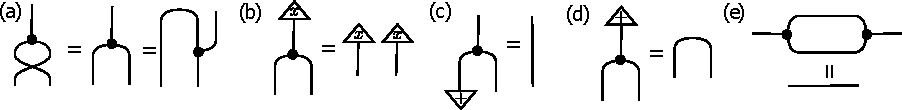
\includegraphics[width=15\xxxscale]{copy-dot}
\end{center}
\end{definition}

\begin{remark}[\COPY-tensors on as generalized delta functions]
 The valence-three \COPY-tensor in terms of components for the case of qubits can be expressed as 
 \be 
 \delta_{ijk} = (1-i)(1-j)(1-k)+ijk, 
 \ee 
 which can be thought of a generalized delta function, where $i,j,k=0,1$.  This can be extended to valence-n \COPY-tensors as 
 \be 
 \delta_{ijk...l} = (1-i)(1-j)(1-k)...(1-l)+ijk...l.
 \ee 
 In figure (e) 
 from Definition \ref{def:copy-prop}, the composition of two \COPY-tensors becomes 
 \be 
 \delta^i_{~jk}\delta^{jk}_{~~m} = \delta^i_{~m}.
 \ee 
We note that the valence-two delta tensor in components is given as 
 \be
 \delta^i_{~j} = 1-(i-j)^2 = (1-i)(1-j)+ij,
 \ee
 where $i,j=0,1$. 
\end{remark}

\begin{myexercise}\label{exercise:rank1}
(Rank-1 projectors). 
Show that a non-trivial operator $P_\star$ is a Schmidt rank-1 projector if and only if it can be written as $\ketbra{\psi}{\psi}$. \\

% \noindent {\bf Solution}. Let us write $P$ in terms of its singular value decomposition $P= UDV^\dagger$.  Assume $P$ is a projector.  Then $P^2 = P$ implies that 
% \begin{equation}\label{eqn:svdP}
% UDV^\dagger UDV^\dagger = UDV^\dagger,
% \end{equation}
% and so $V^\dagger U = \I$ and hence $V = U$.  We  further have from \eqref{eqn:svdP}  that $D^2=D$ and so $\text{spec}\{D\}\in \{0,1\}$. For $D$ rank-1, only a single eigenvalue is non-zero.  The eigenvalues of $D$ are monotonically ordered lexicographically in the standard basis. Hence $D = \ketbra{\bf 0}{\bf 0}$ and so $U\ketbra{\bf 0}{\bf 0}U^\dagger = \ketbra{\psi}{\psi}$. Note that an example of projector that has full rank $k$ is the $k\times k$ identity. One with rank $k-1$ is found considering $\I - \ketbra{a}{a}$. 
\end{myexercise}


\begin{theorem}[Diagrammatic SVD]
\label{theorem:diagrammatic-SVD}
Every operator $A: \hilb{H}_1 \to \hilb{H}_2$ can be
factored into a nonnegative order-one tensor $\sigma$ (unique), an order-three \COPY-tensor
and unitary order-two tensors~$U$ and~$V$:
\begin{center}
 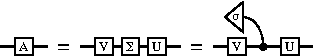
\includegraphics[width=0.7\textwidth]{SVD}
\end{center}
\begin{proof}
Using the SVD, every valence-two tensor $A^i_l$ can be written as
\be 
A^i_l = U^i_j~\Sigma^j_k~V^k_l,
\ee
where $U$ and $V$ are unitary and $\Sigma$ is diagonal and nonnegative
in the standard bases of $\hilb{H}_1$ and $\hilb{H}_2$.
$\Sigma$ can be written as
\be 
\begin{aligned}
\Sigma =& \sum_{j=0}^{\min(d_1, d_2)-1} \sigma_j \ket{j}_2\bra{j}_1, \\
=& \underbrace{\sum_{i=0}^{\min(d_1, d_2)-1} \ket{i}_2 \bra{i}_1}_{Q_{12}}
\underbrace{\sum_{j} \ket{j}_1\bra{jj}_1}_{\COPY}
\underbrace{\sum_k \sigma_k \ket{k}_1}_{\sigma},
\qquad (\text{where}~~\sigma_k \ge 0).
\end{aligned}
\ee 
We have then expressed the tensor $\Sigma$ as a contraction of an
order-one tensor~$\sigma$ with the \COPY-tensor.
The tensor $Q_{12}$ is only necessary if $\hilb{H}_1$ and $\hilb{H}_2$
have different dimension.
\end{proof}
\end{theorem}

\begin{remark}[Eckart-Young-Mirsky Theorem]
The rank of a matrix~$A$ is the number of non-zero singular values it has.
To determine its optimal rank-$r$ approximation (with $r < \text{rank}(A)$), we can turn to a classic theorem by Eckart and Young which was generalized by Mirsky.

Given the SVD, $A = U\Sigma V^\dagger$, we will discard $\text{rank}(A)-r$ smallest singular values in~$\Sigma$ by setting them to zero, obtaining~$\Sigma'$.
This process is often called trimming.

This gives rise to $A' = U\Sigma' V^\dagger$, an approximation of~$A$. 
\begin{theorem}[Eckart-Young-Mirsky] For $m\times m$ matrices $A$, $A'$
\begin{equation}
\lVert A -A' \rVert =  \min_{\text{rank}(\hat{A}) \le r} \lVert A -\hat{A}\rVert,
\end{equation}
for any unitarily invariant matrix norm $\lVert \cdot \rVert$ with $r < \text{rank}(A)$.
\end{theorem}
\marginnote{\emph{\textit{Interested readers can try to get their hands on copies of
C. Eckart and G. Young, ``The approximation of one matrix by another of lower rank,'' Psychometrika 1, (1936)
and
L. Mirsky, ``Symmetric gauge functions and unitarily invariant norms,'' The Quarterly Journal of Mathematics 11:1, 50--59 (1960).}}}
Here $\hat{A}$ is any approximation to $A$ of the same or lesser rank as~$A'$.
This implies that truncating or trimming $\Sigma$ in this way yields as good of an approximation as one can expect.
In the following section, we will specifically consider the induced error for such an approximation.
\end{remark}
% he should be careful on the types of copy however.  
% In fact, copy only is defined if all legs are of the same type.  
% So one can't be larger than the other.  There is no proof there for this being the case, 
% though it is in fact always true that you can 
% split a system using copy with type of the min dimension of the systems you split. 

\begin{corollary}[Diagrammatic Schmidt decomposition]
\label{ex:diagrammatic-Schmidt}
Given a bipartite state $\ket{\psi}$, we use the snake equation to
convert it into a linear map (inside of the dashed region).
Now we apply the SVD as in
Theorem~\ref{theorem:diagrammatic-SVD},
resulting in unitary maps $U$ and $V$, a \COPY{}-tensor and the
order-one tensor~$\sigma$ representing the singular values.
Diagram reorganization leads to the diagrammatic Schmidt decomposition
of~$\ket{\psi}$:
\begin{center}
 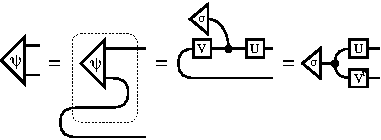
\includegraphics[width=12\xxxscale]{schmidt}
\end{center}
(Sliding $V$ around the cup takes the transpose but
the resulting map is still unitary).
The singular values $\sigma_0, \ldots, \sigma_{d-1}$ in $\sigma$ correspond to
the Schmidt coefficients.
\end{corollary}

\begin{example}[Graphical map-state duality]
 In the figure from Corollary \ref{ex:diagrammatic-Schmidt}, we arrive at an example of map-state duality from \cite{Meznaric2014} as 
 \begin{center}
 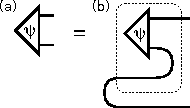
\includegraphics[width=7\xxxscale]{map-state-duality-2}
\end{center}
 In (a) we start with a state $\ket{\psi}$.  We can think of this (vacuously, it would seem) as a state being acted on by the identity operation.  Application of the snake-equation to one of the outgoing wires allows one to transform this into the diagram in (b).  We can think of (b) a Bell state (left) being acted on by a map found from coefficients of the state $\ket{\psi}$.  We have illustrated this map acting on the bell state by a light dashed line around $\ket{\psi}$. 
\end{example}

\begin{definition}[Partition $\chi$]
Given a many-body quantum state, partition the state into two halves and perform the diagrammatic SVD on this system, with respect to this partition.  The term ``$\chi$'' stands for the number of non-zero singular values across a bipartition of a state.  These values are used to compute the entanglement entropy
\eqref{eqn:entropy} of either reduced subsystem.  
\end{definition}

\begin{example}[Entanglement topology]
The most significant topology change occurs when the input state to
the black \COPY-tensor is a copy point --- this causes the diagram to
break into two.  When the input state is a unit for the \COPY-tensor,
the tensor structure is converted to a smooth wire (this is the
maximally entangled case).
\begin{center}
 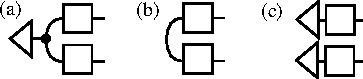
\includegraphics[width=8\xxxscale]{entanglement-topology}
\end{center}
(a) is the general form of a state $\psi = \sum \alpha^i \ket{\varphi_i}\ket{\phi_i}$ with $\chi>1$ and at least two singular values taking different values, that is  $\exists \lambda_i\neq \lambda_j$ for some $i\neq j$.  The state takes the form in (b) iff the singular values in the triangle from (a) all take the same values, so $\lambda_i=\lambda_j$ $\forall i,j$ with clearly $\chi=d$ .  In this case, the state is LU equivalent to a generalized Bell state, in dimension $d$.  The state takes the form in (c) iff the first singular value equals one, which necessarily implies that the remaining singular values are zero.  In such a case, the state is separable and $\chi=1$.   
\end{example}

\begin{corollary}[Diagrammatic state purification]
The diagrammatic SVD from Theorem \ref{theorem:diagrammatic-SVD} gives rise to a diagrammatic representation of state 
purification.  To begin with consider
\begin{center}
 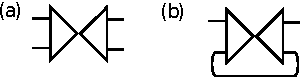
\includegraphics[width=6\xxxscale]{reduced-density-state}
\end{center}
In (a) we have a two-party pure density state $\ket{\psi}\bra{\psi}$ and in (b) we trace 
out one subsystem $\rho'\bydef\text{Tr}_2(\ket{\psi}\bra{\psi})$.  Now consider 
\begin{center}
 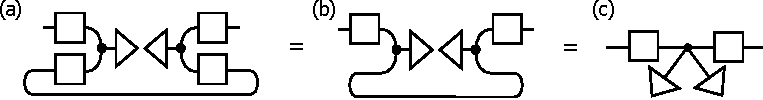
\includegraphics[width=14\xxxscale]{density-states}
\end{center}
(a) is found from applying the diagrammatic SVD to the reduced state $\rho'$.  
(b) follows from applications for simple diagrammatic rewrite rules, allowing the bottom unitaries to cancel. 
This follows from pulling both boxes around the bends, which takes the transpose of each map.  We arrive at $U^{\dagger
  \top}U^\top=(UU^{\dagger})^\top=\I$.
In (c) the \COPY-tensors merge, resulting in multiplication of the singular values stored in the valence-one triangular tensors.  

Alternatively, $\ket{\psi}$ can be seen as a purification of $\rho_1$
(the square roots of the singular values multiply (c) resulting again in
$\rho_1$.) These diagrams translate between a purification of a density
operator and the density operator itself.
\end{corollary}

\section{Matrix Product Factorization of States}\label{sec:mps} 

As a key application of the diagrammatic SVD, we will consider Matrix Product States (MPS), an iterative method to factor quantum states into a linear chain of tensors (see \cite{MPSreview08,TNSreview09}).  We will express this factorization in terms of the diagrammatic SVD \ref{theorem:diagrammatic-SVD}, and our focus will be on exposing the degrees of freedom which are invariant under local groups acting on open tensor legs.  A basis to expand any local unitary invariant of an MPS will be explored in \S~\ref{sec:monomial-mps}.

\begin{remark}
The early work in \cite{2007PhRvL..98v0503G, GESP07} cast measurement based quantum computation into the graphical language of tensor networks.
\end{remark}

\begin{definition}
 Given an $n$-party quantum state $\ket{\psi}$, fully describing this state generally requires an
amount of information (or computer memory) that grows exponentially with~$n$.
If $\ket{\psi}$ represents the state of $n$~qubits,
\be 
\ket{\psi}= \sum_{i j \cdots k}\psi_{i j \cdots k}\ket{i j \cdots k},
\ee 
the number of independent coefficients $\psi_{i j \cdots k}$ in the basis expansion in general would be $2^n$
which quickly grows into a computationally unmanageable number as~$n$ increases.
The goal is to find an alternative representation of~$\ket{\psi}$ which is less data-intensive.
We wish to write $\ket{\psi}$ as 
\begin{equation}\label{eqn:matrix}
\ket{\psi} = \sum_{i j \cdots k} \trace(A_{i}^{[1]} A_{j}^{[2]} \cdots A_{k}^{[n]}) \ket{i j \cdots k},
\end{equation}
where $A_{i}^{[1]}, A_{j}^{[2]}, \ldots, A_{k}^{[n]}$ are indexed sets of matrices and  trace (tr)  closes the boundaries and could be omitted (e.g.~$A_{i}^{[1]}$ and $A_{k}^{[n]}$ are row and column vectors respectively).
Calculating the components of $\ket{\psi}$ then becomes a matter of calculating the products of matrices,
hence the name \emph{matrix product state}.

If the matrices are bounded in size, the representation becomes efficient
in the sense that the amount of information required to describe them is only linear in~$n$.
The point of the method is to choose these matrices such that they provide a good (and compact) approximation to~$\ket{\psi}$.
For instance, if the matrices are at most $\chi$ by $\chi$, the size of the representation scales as~$n d \chi^2$,
where $d$~is the dimension of each subsystem.
\end{definition}

Without loss of generality, we will apply the MPS method to a four-party state, and explain the procedure in terms of three distinct steps.  Consider a quantum state, expressed as a triangle in the Penrose graphical notation with a label $\textbf{1}$ inside and open legs labeled $i,j,k,m$.  
\begin{center}
 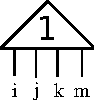
\includegraphics[width=2\xxxscale]{MPS-state}
\end{center}

(Step I). We will now create a partition of the legs of this state, into a first collection containing only leg $i$ and a second collection containing legs $j,k,m$.  We will then apply the diagrammatic SVD across this partition.
The partition is illustrated with the dashed \textit{cut} below in (a).  Figure (b) results from applying the diagrammatic SVD across this partition, factoring the original state with label $\textbf{1}$ in (a) into a valence-two unitary box with label $\textbf{2}$, a valence-one triangle containing the singular values with label $\textbf{3}$, and a 
valence-four triangle with label $\textbf{4}$, all contracted with a \COPY-tensor, as illustrated.  A new internal label (d) for the wire connecting the \COPY-tensor to the valence-four triangle ($\textbf{4}$) was introduced for clarity. (see also Figure \ref{fig:MPS-summary} (a) and (b)). 
\begin{center}
 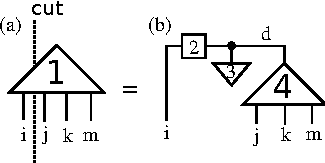
\includegraphics[width=6\xxxscale]{MPS-II}
\end{center}

\begin{remark}[Isometric internal tensors]
 The valence-four triangle tensor in (b) above is actually a unitary map.  The only input leg shown is labeled d.  The other legs are contracted with a fixed basis state $\ket{0}$, from the SVD (a).  We then depict this as the triangle $\textbf{4}$ as in (b).  From the unitarity property, the isometry property follows, as illustrated graphically in (c).  
 \begin{center}
  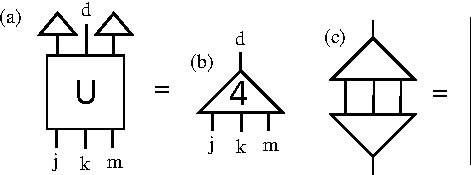
\includegraphics[width=7\xxxscale]{MPS-unitary}
 \end{center}
\end{remark}

\begin{remark}[Contraction of Unitaries]
In tensor network diagrams, two unitaries compose to form unitaries.  In (a) below, we factor a tensor with three legs into an order-two unitary (white box), a black order three \COPY-tensor contracted with an order-one triangle of singular values and an order-four unitary with label $U$.  In (b) we remove $U$ and act on it with an arbitrary order-two tensor.  These compose to form $\widetilde{U}$ which is still unitary.  In a general MPS, unitaries acting on the open legs do not alter the singular values found in a factorization.
\begin{center}
 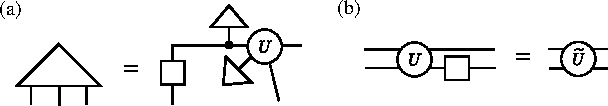
\includegraphics[width=12\xxxscale]{unitary-composition}
\end{center}
\end{remark}


(Step II). To illustrate the next step in the factorization, we will remove the tensor labeled $\textbf{4}$ by breaking the wire connecting it to the \COPY-tensor (a).  We will then partition this separate tensor into two halves, one containing wires $d, j$ the other half wires $k,m$.  This partition is illustrated by placing a dashed line (labeled cut) in (a).   We arrive at the structure in (b), which we have explained in the first step.  (see also Figure \ref{fig:MPS-summary} (b) and (c)).  
\begin{center}
 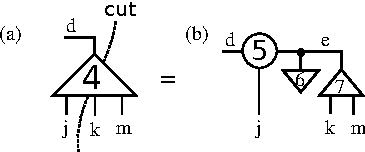
\includegraphics[width=6\xxxscale]{MPS-III}
\end{center}

\begin{remark}[An elementary property of tensor network manipulation]\label{remark:elementary-prop-1}
 It is a fundamental property of tensor network theory that one can remove a portion of a network, alter this removed portion of the network without changing its function, and replace it back into the original network, leaving the function of the original network intact.   
\end{remark}

(Step III).  In the third and final step of the MPS factorization applied to this four-party example, following remark \ref{remark:elementary-prop-1} we first place the tensor we have factored in the second step, back into the original network from the first step, see (a) below.  We then repeat the second step, applied to the triangular isometry tensor, labeled internally with a $\textbf{7}$.  This results in the factorization appearing in (b).  (see also Figure \ref{fig:MPS-summary} (c) and (d)).  
\begin{center}
 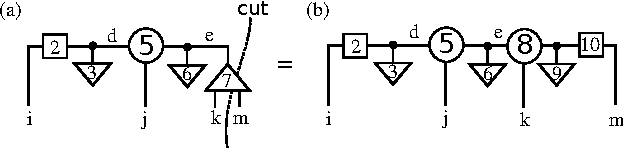
\includegraphics[width=10\xxxscale]{MPS-step-3}
\end{center}

\begin{remark}[Step $n$]
 The iterative method continues in the same fashion as the first three steps, resulting in a factorization of an $n$-party state.  A summary of the MPS factorisation applied to a four-party state is shown in Figure \ref{fig:MPS-summary}. 
\end{remark}

\begin{figure}[t]
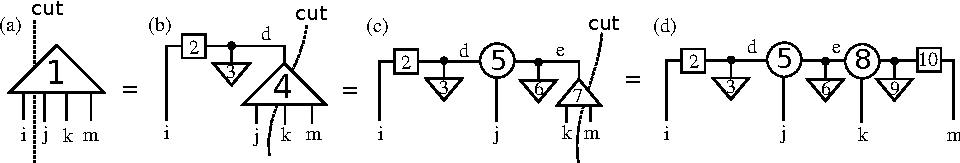
\includegraphics[width=16\xxxscale]{MPS-summary}
\caption{(Diagrammatic summary of steps I, II and III). The quantum state (a) is iteratively factored into the 1D Matrix Product State (d). This procedure readily extends to $n$-body states.}
\label{fig:MPS-summary}
\end{figure}
% \yo{FIXME the figure needs improvement, and the explanation/proof
% too. Explain cut. Explain isometry. Keep dimensions explicit.}
% honestly, if the dims confuse people, there is nothing I can say to help them, since they are fucked any way.  

(Summary). We will now consider Figure \ref{fig:MPS-summary}, which summarizes the factorization scheme. In the steps we have outline, we have factored the Figure \ref{fig:MPS-summary} original state (a) into the MPS in Figure \ref{fig:MPS-summary} (d), in terms of the components listed below.  

\begin{itemize}
 \item[(i)] States (labeled $\textbf{3}$, $\textbf{6}$ and $\textbf{9}$; denoted $\phi_3$, $\phi_6$ and $\phi_9$, respectively): $\phi_3=(\lambda_0,\lambda_1)^\top$, $\phi_6=(\lambda_2,\lambda_3,\lambda_4,\lambda_5)^\top$ and $\phi_9=(\lambda_6,\lambda_7)^\top$.  The $\lambda_i$'s are the singular values across each partition.  The number of non-zero singular values ($\chi$) is given by the minimum dimension of the two parties in the cut.  For the case of qubits, the first outside partition has at most two non-zero entries, and the next inside partition has at most $\14$.   One might also consider the singular values as the eigenvalues of either member of the pair of reduced density matrices found from tracing out either half of a partition.  
 \item[(ii)] Unitary gates (labeled $\textbf{2}$ and $\textbf{10}$; denoted $U_2$ and $U_{10}$, respectively).  
 \item[(iii)] Isometries (labeled $\textbf{5}$ and $\textbf{8}$; denoted $I_5$ and $I_8$ respectively).   The isometry condition describes the tensor relation $I_{jq}^d ~\overline{I}^{jq}_r = \delta ^d_{~r}$.  It is a consequence of the fact that tensors $\15$ and $\18$ arise from unitary gates, as explained in Step II.  The isometry condition plays a more relevant role in structures other than 1D tensor chains.   
\end{itemize}

We note that by appropriately combining neighboring tensors as in Figure \ref{fig:MPS-equation} (a), one recovers the familiar matrix product representation of quantum states \ref{fig:MPS-equation} (b).  Matrix product states are written in equational form as  
\begin{equation}\label{eqn:MPS}
 \psi = \sum_{i,j,k,m} A^{[1]}_i A^{[2]}_j A^{[3]}_k A^{[4]}_m\ket{ijkm}.
\end{equation}
Here $A^{[1]}$ becomes a new tensor formed from the contraction of tensors labeled $\12$, $\13$, and $A^{[2]}$ is a contraction of tensors labeled $\15$ and $\16$, etc. The exact grouping has some ambiguity.  

A utility of our approach Figure \ref{fig:MPS-equation} (a) is that the \COPY-tensor is well defined in terms of purely graphical rewrite identities (as seen in Definition \ref{def:copy-prop}).  These graphical relations allow one to gain insights (into e.g.\ polynomial invariants as will be seen), and to contract portions of tensor networks by hand.
The factorization we present however, allows one to perform many diagrammatic manipulations with ease, and exposes more structure inherent in a MPS.  

\begin{remark}[Data compression]
 The compact representation of an MPS is recovered by picking a cutoff value for the singular values across each partition, or a minimum number of allowed singular values.  This allows one to compress data by truncating the Hilbert space and is at the heart of MPS computer algorithms in current use.  
\end{remark}



\begin{figure}[h]
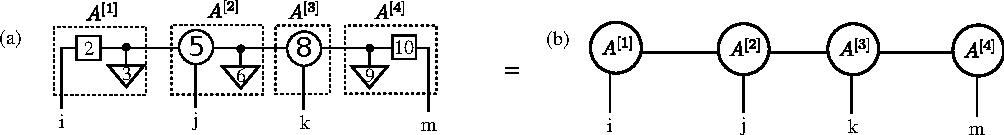
\includegraphics[width=15.5\xxxscale]{MPS-equation}
\caption{Conversion from our notation (a), to conventional MPS notation (b). The factorization methods we have reviewed here allow one to ``zoom in'' and expose internal degree of freedom (a) or ``zoom out'' and expose high-level structure (b). The equational representation of the MPS in (b) is given in \eqref{eqn:MPS}.}
\label{fig:MPS-equation}
\end{figure}

The singular values found from the MPS factorization can be used to form a complete basis to express any quantity related to an MPS that is invariant under local unitary operations.  This includes providing a complete basis to express any entanglement monotone.  %We will explain this next.  



\begin{example}[MPS for the GHZ state]\label{ex:mps-ghz}
The standard MPS representation of the Greenberger-Horne-Zeilinger (GHZ) state is given as \marginnote{Daniel {\bf G}reenberger, Michael {\bf H}orne and Anton {\bf Z}eilinger first studied what is now named the {\sf GHZ}-state in 1989 \cite{GHZ}.}
\be\label{eqn:ghzMPS}
\ket{\text{GHZ}} = \frac{1}{\sqrt{2}}\trace\left( \begin{array}{cc}
\ket{0} & 0 \\
0 & \ket{1} \end{array} \right)^{n}=
\frac{1}{\sqrt{2}}(\ket{00\ldots 0}+\ket{11\ldots 1}).
\ee
Alternatively, we may use a quantum circuit made of \CNOT{} gates to construct
the GHZ state,
and then use the rewrite rules employed in Examples 
\ref{ex:circuits-2} and \ref{ex:state-prep}
%\marginnote{PS} 
to recover the familiar MPS comb-like structure consisting of \COPY{} tensors:
\begin{center}
   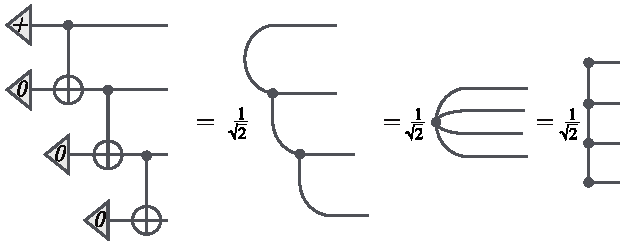
\includegraphics{mps-ghz}
\end{center}


Diagrammatically, any tensor network formed from connected \COPY{}-tensors reduces to a single dot
with the appropriate number of input and output legs.
Hence one might write the n-party \GHZ-state as 
\be 
\ket{\text{GHZ}} = \frac{1}{\sqrt{2}}\sum_{ijk\ldots l} \COPY^{ijk\ldots l}\ket{ijk\ldots l}.
\ee 
\end{example}

\begin{example}[MPS for the W state]\label{ex:w-state}
Like the GHZ state from Example \ref{ex:mps-ghz}, the $n$-qubit W~state ($n\geq 3$) has the following MPS representation:
\be\label{eqn:wnMPS1}
\begin{aligned}
\ket{W}
=&
\frac{1}{\sqrt{n}}
\begin{pmatrix} \ket{1} & \ket{0} \end{pmatrix}
\left( \begin{array}{cc}
\ket{0} & 0 \\
\ket{1} & \ket{0} \end{array} \right)^{n-2}
\begin{pmatrix} \ket{0}\\ \ket{1} \end{pmatrix},\\
=&
\frac{1}{\sqrt{n}} \left(
\ket{10\ldots 0}+\ket{010\ldots 0}+\ldots +\ket{0\ldots 01}
\right).
\end{aligned}
\ee
\end{example}


\subsection*{Invariant Basis for Matrix Product States}\label{sec:monomial-mps}

We will consider generating a full monomial basis in terms of the singular values found in the factorization of Matrix Product States.  The monomial basis is generated as a matter of convenience and can be used to define a basis for entanglement monotones.   In fact, we will see that the diagrammatic factorization can be used to prove that certain tensor contractions give rise to certain invariants, which allow one to calculate quantities of interest, such as the concurrence or R\'{e}nyi entropy.  These tensor contractions are not dependent on the factorization method used, and are general. The diagrammatic SVD will be used to prove that the contraction of certain tensors, results in an expression that is in terms of the singular values.  
%\yo{FIXME also here, why a monomial basis?}
% check above and see if you agree to it? 

Our objective will be to develop tensor contractions that evaluate to specific quantities of interest.  These quantities of interest will be invariants of the local unitary group.  
Such invariants have expansions in terms of the singular values of reduced density operators.  We will use tensor network contractions to evaluate a full basis that can be used to expand any 
function of the singular values.  This includes quantities of interest such as concurrence and R\'{e}nyi Entropy.  

For the general case, one can, for instance, form a polynomial basis using the elementary symmetric polynomials by combining the $\lambda$ as   
\begin{equation}
 S_1 = \sum_i \lambda_i,
\end{equation}

\begin{equation}
 S_2 = \sum_{i\neq j} \lambda_i\lambda_j,
\end{equation}

\begin{equation}
 S_3 = \sum_{i\neq j\neq k} \lambda_i\lambda_j\lambda_k, 
\end{equation}
and so on.  Such polynomials are used to calculate the d-concurrence, see Definition \ref{def:d-concurrence}.  
Any polynomial in the $S$'s is necessarily a local unitary invariant.  

Another basis of interest, is the basis formed by summed powers of the singular values
\be 
B_n = \sum_i \lambda_i^n,
\ee 
which is of great interest to evaluate R\'{e}nyi's entropy, see Definition \ref{def:R\'{e}nyi}.  
The polynomial $B_2$ is related to the concurrence measure of entanglement in Definition \ref{def:concurrence}.  
For the case of qubits, $B_2=\lambda_0^2 + \lambda_1^2$ which is greater than zero iff the state is entangled.
Increase $n$, pattern continues up to $B_d$.  $B_d$ being greater than
zero implies that $B_n\geq 0$ for all $1\leq n \leq d$.  In addition,
$B_n=0$ implies that $B_k=0$ for all $n\leq k \leq d$.

We will first recall the definition of the concurrence (see \cite{concurrence}) and then the definition of R\'{e}nyi's Entropy (see for instance \cite{Renyi}). 
These quantities are of physical interest.  As will be shown, they can be calculated by contracting specific tensor networks.  


\begin{definition}[The concurrence]\label{def:concurrence}
The concurrence of a pure bipartite normalized state $\ket{\psi}$ is defined as 
%(see example \ref{ex:concurrence}) 
\be 
C(\ket{\psi}) := \sqrt{\frac{d}{d-1}(1-\text{Tr}\rho^2)},
\ee 
where $\rho$ is obtained by tracing over one subsystem.  The factor $\sqrt{d/(d-1)}$ ensures that $0\leq C(\ket{\psi}) \leq 1$.   
\end{definition}

\begin{remark}[Tensor contractions for the concurrence]
 We will contract tensor networks that evaluate to $B_2=\text{Tr}(\rho^2)$ and these hence can be used to evaluate the concurrence.  
\end{remark}

\begin{definition}[The $d$-concurrence]\label{def:d-concurrence}
 Consider a d $\times$ d-dimensional bipartite pure state $\ket{\psi}$ with Schmidt numbers 
 $\lambda:=(\lambda_0, \lambda_1, ..., \lambda_{d-1})$ the d concurrence monotones, $C_k(\ket{\psi})$, $k=1,2,...,d$, of the state $\ket{\psi}$ are defined as follows
 \be 
 C_k(\ket{\psi}) := \left(\frac{S_k(\lambda_0, \lambda_1, ..., \lambda_{d-1})}{S_k(1/d,1/d,...1/d)}\right)^{1/k},
 \ee  
 where $S_k$ is the kth elementary symmetric polynomial.  
\end{definition}

\begin{definition}[The R\'{e}nyi Entropy]\label{def:R\'{e}nyi}
 The R\'{e}nyi entropy of order $\alpha$ is defined to be 
 \be 
S_\alpha := \frac{1}{1-\alpha} \ln\sum \lambda_i^\alpha,  
 \ee  
and in the limit $\alpha \rightarrow 1$ 
\be 
E=\lim_{\alpha \rightarrow 1}S_\alpha = -\sum_i \lambda_i \ln \lambda_i.
\ee 
\end{definition}

\begin{remark}[Lower bounds on Entropy]
Consider a quantum circuit representing a quantum qubit state (a quantum circuit is a tensor network where all wires have bond dimension $2$).  
Partition this state into a block of $k$-spins and a block of $m$-spins. Let the number of wires connecting the two blocks be given as $l$.  Then 
\be 
E\leq \min\{k,m,l\}, 
\ee 
where all the wires are of bond dimension $2$. 
\end{remark}


In the remaining sections, we will consider tensor networks that enable the evaluation of the quantities of interest we have mentioned here. 
At the heart of the MPS method, is the factorization of a state into two halves.  Our diagrammatic SVD allows one to prove that certain networks contract to 
quantities that can readily be related to the concurrence or R\'{e}nyi's entropy.  In what follows, we build examples for bipartite states.  These generally apply to Matrix Product States 
by considering partitions.  In fact, in the diagrammatic language, it is often useful to group $k$-wires into one wire, for the purpose of manipulation \cite{BB11}.  


\section{Numerical Tensor Network Algorithms and Packages} 

This book is focused on graphical reasoning and the applications of tensor networks to quantum information science.  A primary driving force behind tensor network applications is numerical algorithms for condensed matter physics application.  This is not our main focus, however. 

However, no book would be complete without touching on these important numerical applications.  Indeed, we have described several tensor contractions which can be utilized to solve counting problems (see \S~\ref{part:count}).  And to simulate quantum systems using matrix product states (Part \ref{sec:mps}). 

Those reading this text that want to explore the numerical application of these ideas should be aware of both open source software packages and papers that describe in detail the most effective tensor contraction algorithms.  That is precisely the objective of this appendix.  

\subsection{Online Resources Describing Tensor Network Software Implementations}
Several webpages are devoted to listing papers and tensor contraction algorithms.  Here we provide a short listing of those papers which go into more detail and are of a primary software centric focus.  We have done our best to be as inclusive as possible, however this list is merely an editors pick and is not designed to be comprehensive. 

\begin{itemize}
  \item[1.] {\sf \bf Resource}. \hfill {\it TensorNetwork.ORG}  \\ 
    {\sf \bf Brief description}. An open-source `living' article containing many tensor network resources, applications, and software.\\ 
{\sf \bf Link}. \url{https://tensornetwork.org} \\
{\sf \bf List of Software Packages}. \url{http://tensornetwork.org/software}

\item[2.] {\sf \bf Resource}. \hfill {\it Tensors.NET} \\ 
{\sf \bf Brief description}. A collection of resources, including links to software, tutorials and code in several languages. \\
{\sf \bf Link}. \url{https://www.tensors.net}
\end{itemize}


\subsection{Open Source Tensor Network Software Packages} 
Software packages and programs to do various tensor contractions and related tasks is increasingly available in a variety of languages.  This includes TEBD programs as well as others.  Here we have done our best to include an active and up to date listing of the main packages.  It was last updated \today.  As software packages can appear and also become inactive at any time, a more updated listing of available packages can be currently be found at \url{http://tensornetwork.org/software}. 

We have attempted to list some of the most common packages below. See also {\bf QUIMB}, which is fully featured and aimed at applications in physics; {\bf TenPy} is known to be a small library but with very good MPS codes; {\bf Cyclops}, {\bf TT-Toolbox}, {\bf Tensor Toolbox} are more focused on the {\it tensor train} formulation of MPS~\cite{Oseledets2011} and on decompositions such as CP ({\it tensor rank decomposition} or {\it canonical polyadic decomposition}). 

\begin{itemize}
\item[1.] {\sf \bf Title of package}.\hfill {\it ITensor} \\
{\sf \bf Language}. C++\\ 
{\sf \bf Brief description}. ITensor or Intelligent Tensor is well featured tensor network library implementing a bit of everything out of the box.\\
{\sf \bf Status}. Active (version 3.1.1) \\
{\sf \bf Link}. \url{http://itensor.org} 

    \item[2.] {\sf \bf Title of package}.\hfill {\it TNT} \\
{\sf \bf Language}. Various\\ 
{\sf \bf Brief description}. The TNT library contains highly optimised routines for manipulating tensors and routines that can be used to build the most common tensor network algorithms \cite{2017JSMTE..09.3102A}.\\
{\sf \bf Status}. Active \\
{\sf \bf Link}. \url{http://www.tensornetworktheory.org} 

\item[3.] {\sf \bf Title of package}.\hfill {\it TensorNetwork} \\
{\sf \bf Language}. Python\\ 
{\sf \bf Brief description}. A Google/X package for tensor networks described in \cite{2019arXiv190501330R} and related to Google's popular tensor flow package (\url{https://www.tensorflow.org}). \\ 
{\sf \bf Status}. Active \\
{\sf \bf Github}. \url{https://github.com/google/tensornetwork} 

\item[4.] {\sf \bf Title of package}.\hfill {\it Quantomatic} \\
{\sf \bf Language}. Python\\ 
{\sf \bf Brief description}. A diagrammatic proof assistant supporting reasoning with diagrammatic languages with applications to tensor networks \cite{Dixon2010, Kissinger2014}. \\ 
{\sf \bf Status}. Active \\
{\sf \bf Github}. \url{https://quantomatic.github.io} 






\end{itemize}

\section{Problems} 

\begin{myexercise}[Tensor products, Density operators, Singular values and purification]\label{exercise:svd1}
Let $\psi = \ket{001}+\ket{010}+\ket{100}$ be a state in $\hilb H_1\otimes\hilb H_2$ with $\dim(\hilb H_1)=2$ and $\dim(\hilb H_2)=4$, and let  
\begin{equation}
 V = \left(
\begin{array}{cccc}
 0 & 1 & 0 & 0 \\
 \frac{1}{\sqrt{2}} & 0 & 0 & -\frac{1}{\sqrt{2}} \\
 \frac{1}{\sqrt{2}} & 0 & 0 & \frac{1}{\sqrt{2}} \\
 0 & 0 & 1 & 0
\end{array}
\right).
\end{equation}
\begin{itemize}
 \item[(i)] By writing $\phi = \sum_{ij}C_{ij}\ket{i}\ket{j}$, where $\ket{i}\in\hilb H_1$, $\ket{j}\in\hilb H_2$ are both orthonormal basis, state the values of $i\in\{0,1\},j\in\{0,1,2,3\}$ that correspond to non-zero coefficients of $C_{ij}$ and hence express $\psi$ in the basis $\ket{i},\ket{j}$.    
  \item[(ii)]  Write the $2\times 4$ matrix ${\bf C}=(C_{ij})_{ij}$ and show that ${\bf C}{\bf C}^\dagger$ and ${\bf C}^\dagger {\bf C}$ are (non-normalized) density operators, equivalent to $\rho_1$, $\rho_2$ found by tracing over the systems $\hilb H_1$ and $\hilb H_2$ respectively.  (Here the adjoint $\dagger$ means matrix conjugate transpose.)
 \item [(iii)] From the singular value decomposition, one can write ${\bf C}=U\Sigma V^\dagger$.  For $V$ given above, and $U$ the $2\times 2$ identity matrix, find the $2\times 4$ matrix of singular values $\Sigma$.  
 \item[(iv)] Find purifications for $\rho_1$ and $\rho_2$ (other than $\psi$).  
\end{itemize}
\end{myexercise} 
%%%%%%%%%%%%%%%%%%%%%%%%%%%%%%%%


\begin{myexercise}(Lie product formula---a.k.a.~Trotter-Suzuki decomposition). Show that 
\begin{equation}
e^{A + B}=\lim_{k\rightarrow \infty} \left(e^{A/k}e^{B/k} \right)^k
\end{equation}
for Hermitian matrices $A$ and $B$. 
\end{myexercise}

\begin{myexercise}
The Schmidt number of $\ket{\psi}^{AB}$---denoted Sch($\psi$)---is the rank of the reduced density matrix $\rho_A = \Tr_B(\ketbra{\psi}{\psi})$ where rank of a Hermitian operator is defined as the dimension of its support. 
%\end{myexercise}
%\begin{myexercise}
Let $\ket{\psi} = \alpha \ket{\phi} + \beta \ket{\gamma}$ and prove that 
\begin{equation}
\text{Sch}(\psi)\geq \|\text{Sch}(\phi) - \text{Sch}(\gamma)\|_1
\end{equation} 
\end{myexercise}

\begin{definition}
A {\it multiset} is a modification of a set allowing multiple instances for each element.
\end{definition}

\begin{definition}
 Denote by $\text{Spec}\{A\}$ the multisetset of eigenvalues of square matrix $A$. 
\end{definition}

\begin{myexercise}[Jacobson's Lemma]\label{prob:spec}
Let non-negative $A,B \in \mathcal{L}(\mathbb{C}_n)$.  Show equality of the non-zero elements in the multisets as $\text{Spec}\{AB\}=\text{Spec}\{BA\}$. 
\end{myexercise}

\begin{myexercise}
A matrix $A\in \mathcal{L}(\mathbb{C}_n)$ is non-negative ($A\geq 0$) if
\begin{equation}
    \bra{\psi}A\ket{\psi}\geq 0
\end{equation}
$\forall \psi \in \mathbb{C}_n$. Show that $A\geq 0$ implies the existence of a unique $B$ such that $B^2=A$.
\end{myexercise}

\begin{myexercise}
Let Hermitian $A,B \in \mathcal{L}(\mathbb{C}_n)$. Now suppose that $A^2 = A$ and $B^2=B$ and further that $\{A, B\}=0$.  Let $\|\psi\|_2=1$ and show that 
\begin{equation}
    \bra{\psi}A\ket{\psi}^2 + \bra{\psi}B\ket{\psi}^2\leq 1
\end{equation}
\end{myexercise}

\begin{myexercise}
Consider 
\begin{equation}
\rho = \frac{1}{4}(\I + X\otimes X -Y\otimes Y)
\end{equation} 
and use Lagrange multipliers to find $\|\rho \|_\infty$. 
\end{myexercise}

\begin{myexercise}
Let density operator $\rho^{AB}$ represent the state of a qubit pair (A, B) and define the {\it spin-flipped} density matrix as 
\begin{equation}
    \tilde{\rho}^{AB} = (Y\otimes Y) \bar{\rho}^{AB}(Y\otimes Y)
\end{equation}
where $\bar{\rho}$ is complex conjugate of $\rho$ in the standard basis.  As $\rho^{AB}$, $\tilde{\rho}^{AB}\geq 0$, so is their non-Hermitian product (Problem \eqref{prob:spec}). Consider $\psi$ as the two-qubit Bell state and $\rho = \ketbra{\psi}{\psi}$.  Find the eigenvalues of $\rho \tilde{\rho}$. 
\end{myexercise}




